\section{геометрия решения}
1. \begin{figure}[ht!]
\center{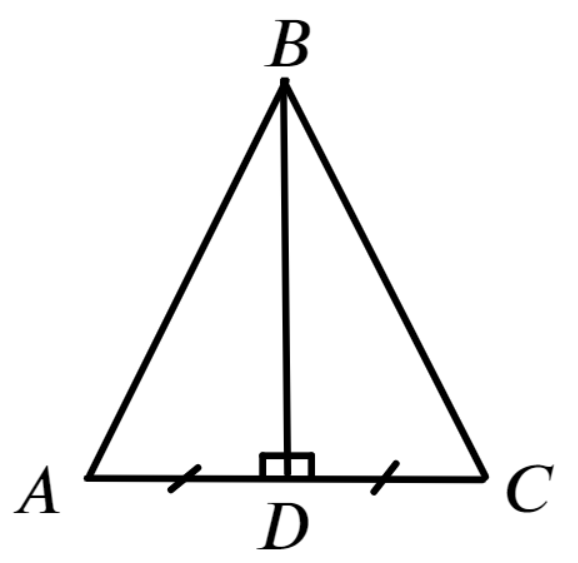
\includegraphics[scale=0.35]{g1.png}}
\end{figure}\\
$\left.\begin{array}{l}AD=DC\text{ т.к. }BD\text{ медиана,}\\
\angle ADB=\angle CDB=90^\circ \text{ т.к. }BD\text{ высота,}\\
BD - \text{ общая.}   \end{array}\right\}\Rightarrow
\Delta ADB=\Delta CDB\text{ по I признаку }\Rightarrow BA=BC\text{ ч.т.д.} $\\
2.  \begin{figure}[ht!]
\center{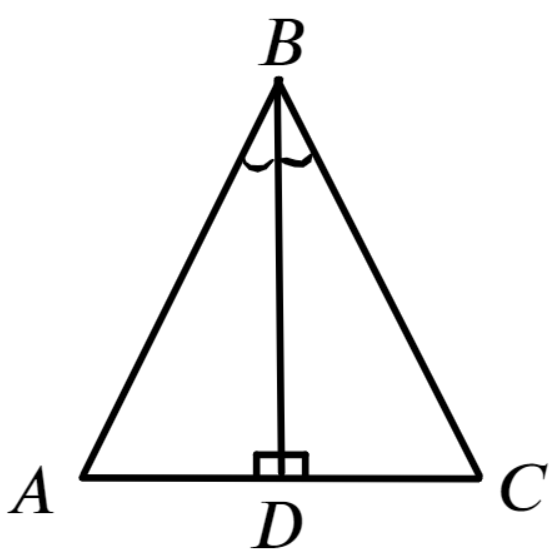
\includegraphics[scale=0.35]{g2.png}}
\end{figure}\\
$\left.\begin{array}{l}\angle ABD=\angle CBD\text{ т.к. }BD\text{ биссектриса,}\\
\angle ADB=\angle CDB=90^\circ \text{ т.к. }BD\text{ высота,}\\
BD - \text{ общая.}   \end{array}\right\}\Rightarrow
\Delta ADB=\Delta CDB\text{ по II признаку }\Rightarrow BA=BC\text{ ч.т.д.} $\\
3. \begin{figure}[ht!]
\center{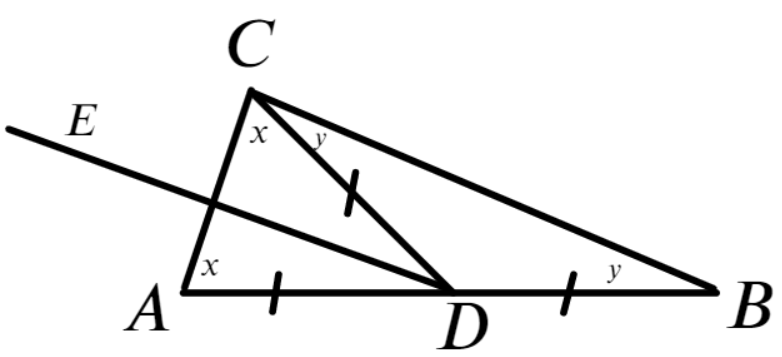
\includegraphics[scale=0.35]{g3.png}}
\end{figure}\\
Треугольники $ADC$ и $BDC$ являются равнобедренными, значит в них углы при основании равны. Обозначим $\angle CAD=\angle ACD=x,\ \angle DBC=\angle BDC=y.$ Тогда выразим сумму углов треугольника $ABC:\ 2x+2y=180^\circ,\ x+y=90^\circ\Rightarrow BC \perp AC\Rightarrow DE\perp AC,$ ч.т.д. (т.к. $DE\parallel BC$)\\
4. \begin{figure}[ht!]
\center{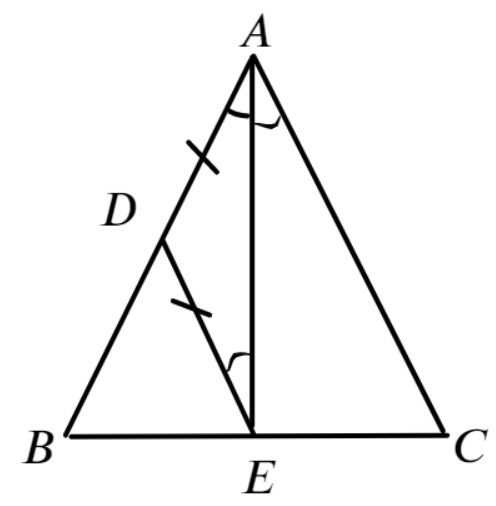
\includegraphics[scale=0.35]{g4.png}}
\end{figure}\\
Треугольник $DAE$ является равнобедренным $(AD=DE),$ значит углы при основании равны: $\angle DAE=\angle DEA.$ Прямые $DE$ и $AC$ параллельны, $AE$ секущая, значит  $\angle DEA=\angle EAC$ как накрест лежащие. Поэтому $\angle DAE=\angle EAC,$ то есть $AE$ является биссектрисой угла $A,$ а поэтому и высотой (так как треугольник $ABC$ равнобедренный). Значит, $AE\perp BC.$\\
5. \begin{figure}[ht!]
\center{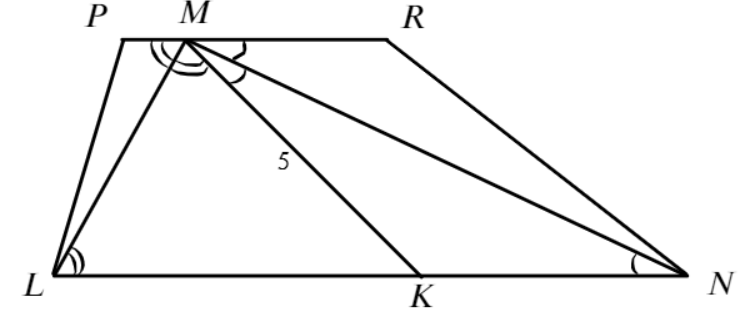
\includegraphics[scale=0.35]{g5.png}}
\end{figure}\\
Прямые $PR$ и $LN$ параллельны, а $LM$ и $MN$ --- секущие, значит $\angle PML = \angle MLK,$  $\angle RMN= \angle MNK$ как накрест лежащие. $MN$ и $ML$ являются биссектрисами, поэтому $\angle PML = \angle LMK,$ $ \angle RMN= \angle NMK.$ Поэтому у треугольников $LMK$ и $NMK$ равны углы при основаниях, а значит они равнобедренные и $LK=MK=5,\ KN=MK=5,$ откуда $LN=LK+KN=5+5=10.$\\
6. \begin{figure}[ht!]
\center{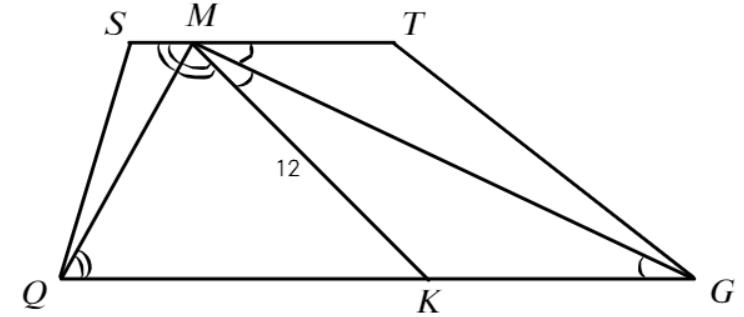
\includegraphics[scale=0.35]{g6.png}}
\end{figure}\\
Прямые $ST$ и $QG$ параллельны, а $QM$ и $MK$ --- секущие, значит $\angle SMQ = \angle MQK,$  $\angle TMG= \angle MGK$ как накрест лежащие. $MG$ и $MQ$ являются биссектрисами, поэтому $\angle SMQ = \angle QMK,$ $ \angle TMG= \angle GMK.$ Поэтому у треугольников $QMK$ и $GMK$ равны углы при основаниях, а значит они равнобедренные и $QK=MK=12,\ KG=MK=12,$ откуда $QG=QK+KG=12+12=24.$\\
7. \begin{figure}[ht!]
\center{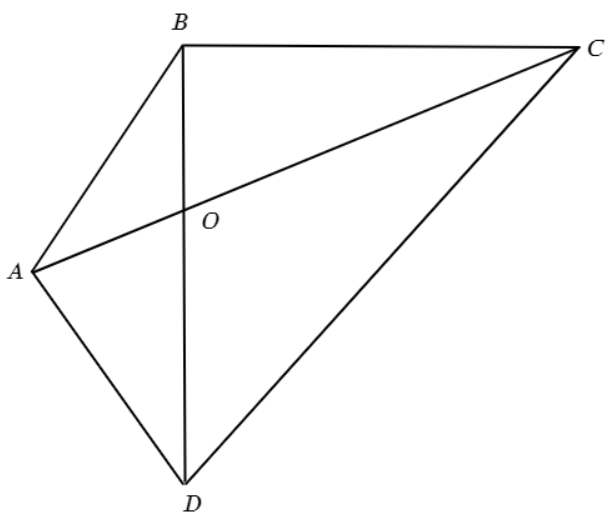
\includegraphics[scale=0.35]{g7.png}}
\end{figure}\\
Запишем четыре неравенства треугольника: $AO+OD>AD,\ BO+AO>AB,\ BO+OC>BC,\ OC+OD>CD.$ После сложения этих неравенств получим $2AO+2OC+2BO+2OD>AB+BC+CD+AD,\ 2(AC+BD)>P,\ AC+BD>\cfrac{P}{2},$ ч.т.д.\\
8. \begin{figure}[ht!]
\center{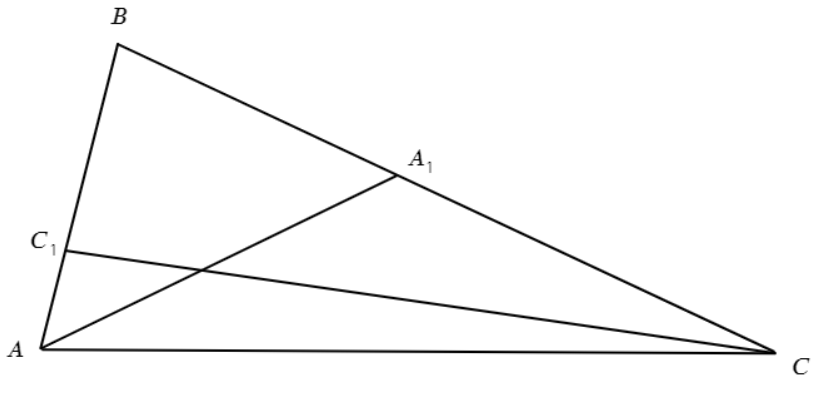
\includegraphics[scale=0.35]{g8.png}}
\end{figure}\\
Запишем четыре неравенства треугольника: $AB+BA_1>AA_1,\ AC+CA_1>AA_1,\ BC+BC_1>CC_1,\ AC+AC_1>CC_1.$ После сложения этих неравенств получим
$AB+AC+BC+AC+BA_1+CA_1+BC_1+AC_1>2AA_1+2CC_1,\ 2P>2AA_1+2CC_1,\ P>AA_1+CC_1,$ ч.т.д.\\
9. \begin{figure}[ht!]
\center{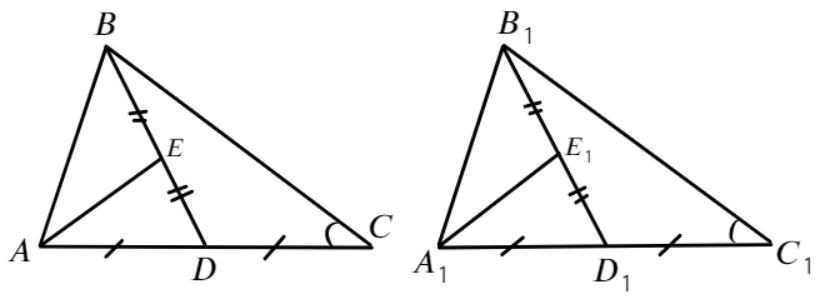
\includegraphics[scale=0.35]{g9.png}}
\end{figure}\\
$\left.\begin{array}{l}BC=B_1C_1,\\
\angle C=\angle C_1,\\
DC=\frac{1}{2}AC=\frac{1}{2}A_1C_1=D_1C_1  \end{array}\right\}\Rightarrow
\Delta BDC=\Delta B_1D_1C_1\text{ по I признаку }\Rightarrow $\\$\Rightarrow ED=\frac{1}{2}BD=\frac{1}{2}B_1D_1=E_1D_1,\ \angle EDA=180^\circ-\angle BDC=180^\circ-\angle B_1D_1C_1=\angle E_1D_1A_1.$\\
$\left.\begin{array}{l}AD=\frac{1}{2}AC=\frac{1}{2}A_1C_1=A_1D_1,\\
\angle EDA=\angle E_1D_1A_1,\\
ED=E_1D_1  \end{array}\right\}\Rightarrow \Delta AED=\Delta A_1E_1D_1\text{ по I признаку }\Rightarrow AE=A_1E_1,$ ч.т.д.\\
10. \begin{figure}[ht!]
\center{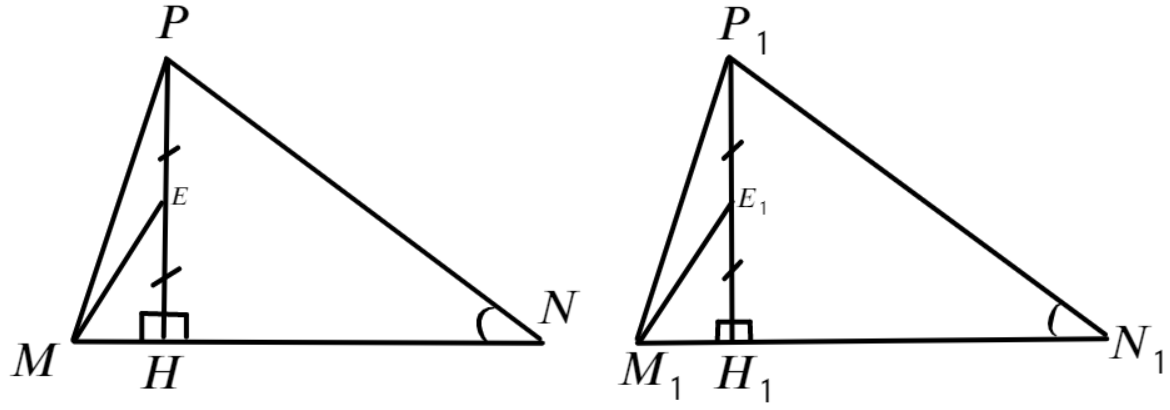
\includegraphics[scale=0.35]{g10.png}}
\end{figure}\\
$\left.\begin{array}{l}PN=P_1N_1,\\
\angle N=\angle N_1. \end{array}\right\}\Rightarrow
\Delta PNH=\Delta P_1N_1H_1\text{ по гипотенузе и острому углу }\Rightarrow $\\$\Rightarrow EH=\frac{1}{2}PH=\frac{1}{2}P_1H_1=E_1H_1,\ MH=MN-HN=M_1N_1-H_1N_1=M_1H_1.$\\
$\left.\begin{array}{l}EH=E_1H_1,\\
MH=M_1H_1  \end{array}\right\}\Rightarrow \Delta MEH=\Delta M_1E_1H_1\text{ по двум катетам }\Rightarrow ME=M_1E_1,$ ч.т.д.\\
11. \begin{figure}[ht!]
\center{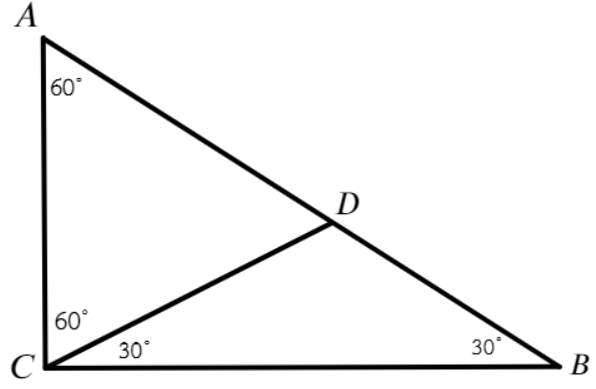
\includegraphics[scale=0.35]{g11.png}}
\end{figure}\\
Треугольник $ACD$ равносторонний, значит все его углы равны $60^\circ.$ Тогда $\angle DCB=\angle C-\angle ACD=90^\circ-60^\circ=30^\circ,\ \angle DBC=180^\circ-\angle A-\angle C=180^\circ-60^\circ-90^\circ=30^\circ.$ Поэтому в треугольнике $BCD$ равны углы при основании $BC$ и он является равнобедренным, ч.т.д.\\
12. \begin{figure}[ht!]
\center{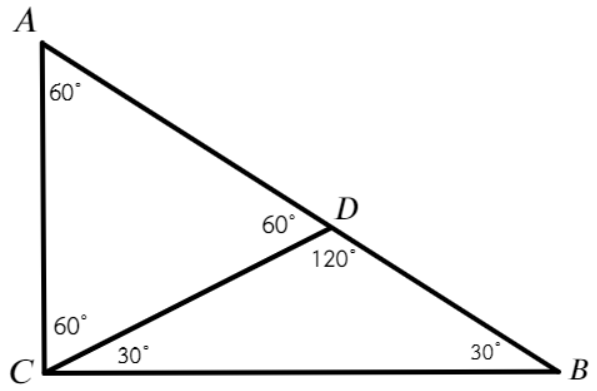
\includegraphics[scale=0.35]{g12.png}}
\end{figure}\\
Треугольник $BCD$ равнобедренный с углом $120^\circ,$ значит углы при основании $BC$ равны $(180^\circ-120^\circ):2=30^\circ.$ Тогда $\angle ACD=\angle C-\angle DCB=90^\circ-30^\circ=60^\circ,\ \angle CAD=180^\circ-\angle C-\angle B=180^\circ-90^\circ-30^\circ=60^\circ,\ \angle CDA=180^\circ-\angle CDB=180^\circ-120^\circ=60^\circ,$
значит треугольник $ACD$ является равносторонним, ч.т.д.\\
13. \begin{figure}[ht!]
\center{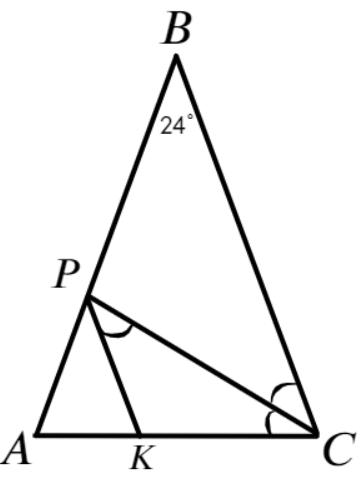
\includegraphics[scale=0.35]{g13.png}}
\end{figure}\\
Треугольник $ABC$ равнобедренный, поэтому $\angle C=(180^\circ-24^\circ):2=78^\circ.$ Так как $CP$ является биссектрисой, $\angle ACP=\angle BCP=78^\circ:2=39^\circ.$ Прямые $BC$ и $PK$ параллельны, $CP$ секущая, поэтому углы $KPC$ и $BCP$ равны как накрест лежащие, откуда $\angle KPC=39^\circ.$\\
14. \begin{figure}[ht!]
\center{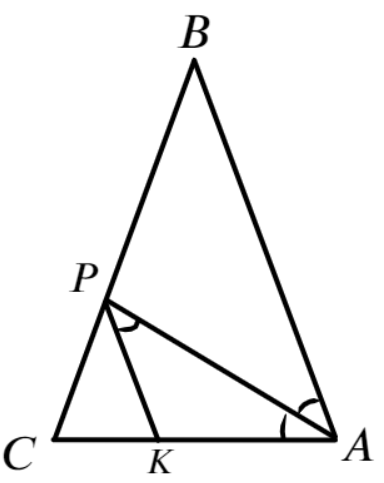
\includegraphics[scale=0.35]{g14.png}}
\end{figure}\\
Треугольник $ABC$ равнобедренный, поэтому $\angle A=\angle C =72^\circ.$ Так как $AP$ является биссектрисой, $\angle PAC=\angle PAB=72^\circ:2=36^\circ.$ Прямые $AB$ и $PK$ параллельны, $AP$ секущая, поэтому углы $KPA$ и $PAB$ равны как накрест лежащие, откуда $\angle KPA=36^\circ.$\\
15. Да, существует. На картинке изображён один из возможных примеров.
\begin{figure}[ht!]
\center{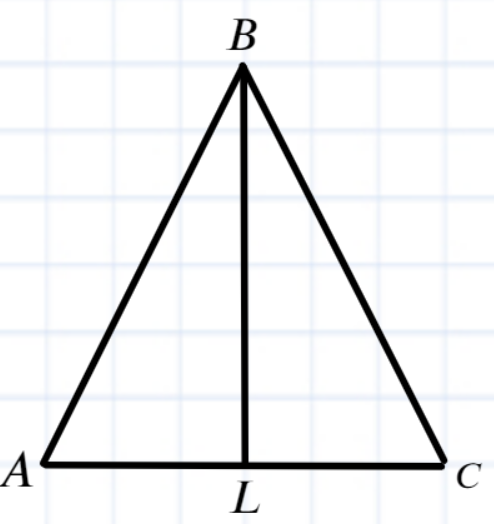
\includegraphics[scale=0.35]{g15.png}}
\end{figure}\\
16. Нет, неверно. На картинке изображён один из возможных примеров.
\begin{figure}[ht!]
\center{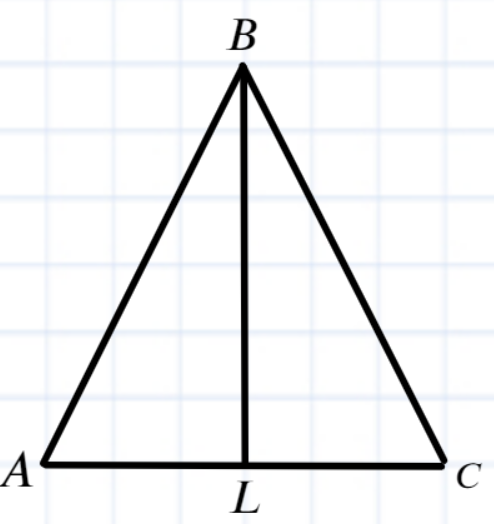
\includegraphics[scale=0.35]{g15.png}}
\end{figure}\newpage\noindent
17. \begin{figure}[ht!]
\center{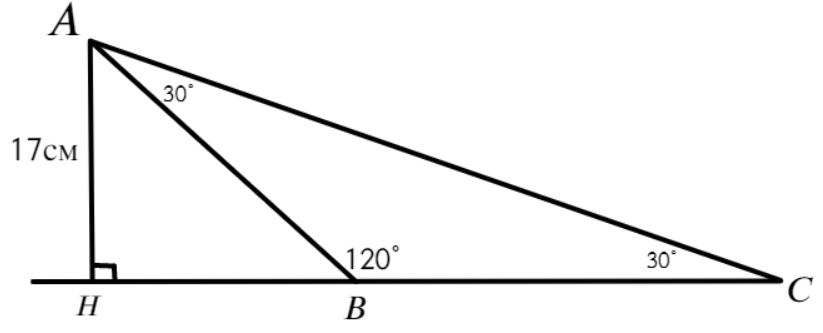
\includegraphics[scale=0.35]{g17.png}}
\end{figure}\\
Углом в $120^\circ$ может быть только угол при вершине, тогда углы при основании треугольника равны $(180^\circ-120^\circ):2=30^\circ.$ Поэтому в прямоугольном треугольнике $AHC$ катет $AH$ лежит напротив угла $30^\circ,$ а значит равен половине гипотенузы $AC.$ Таким образом, $AC=2\cdot17=34$ см.\\
18. \begin{figure}[ht!]
\center{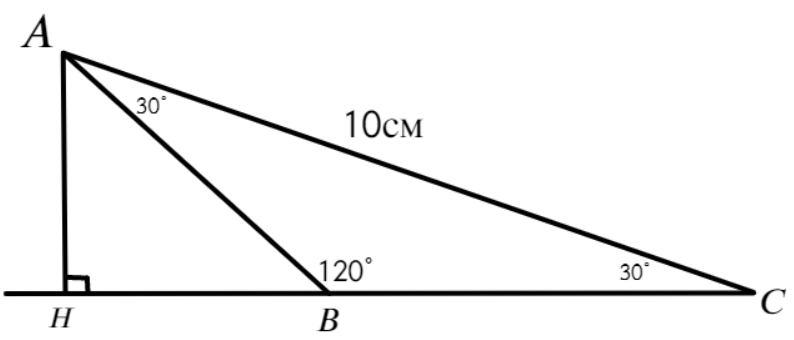
\includegraphics[scale=0.35]{g18.png}}
\end{figure}\\
Углом в $120^\circ$ может быть только угол при вершине, тогда углы при основании треугольника равны $(180^\circ-120^\circ):2=30^\circ.$ Поэтому в прямоугольном треугольнике $AHC$ катет $AH$ лежит напротив угла $30^\circ,$ а значит равен половине гипотенузы $AC.$ Таким образом, $AH=10:2=5$ см.\\
19. Да, можно. На картинке изображён один из возможных примеров.
\begin{figure}[ht!]
\center{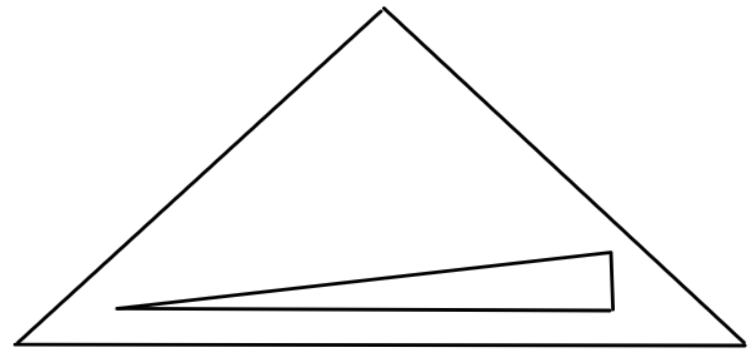
\includegraphics[scale=0.35]{g19.png}}
\end{figure}\\
20. Да, можно. Представим, что две вершины внутреннего треугольника и левая вершина внешнего треугольника лежат на окружности радиусом 566 с центром в нижней вершине.
\begin{figure}[ht!]
\center{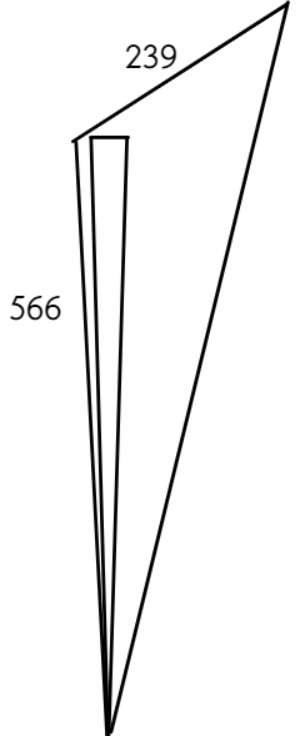
\includegraphics[scale=0.35]{g20.png}}
\end{figure}\newpage\noindent
21. \begin{figure}[ht!]
\center{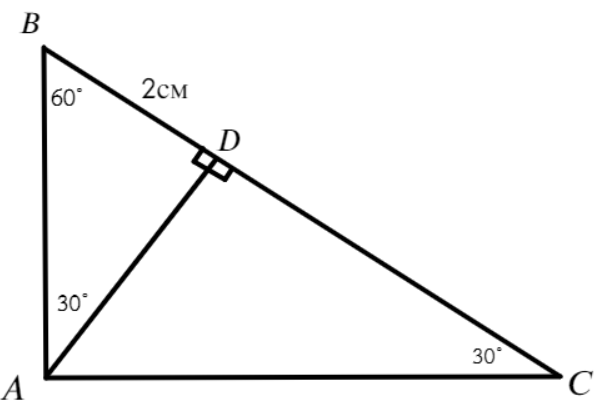
\includegraphics[scale=0.35]{g21.png}}
\end{figure}\\
$\angle BAD=\angle C=90^\circ-\angle B=90^\circ-60^\circ=30^\circ.$ В прямоугольном треугольнике $ABD$ катет $DB$ лежит напротив угла в $30^\circ,$ а значит гипотенуза $AB=2\cdot2=4$см. В прямоугольном треугольнике $ABC$ катет $AB$ лежит напротив угла в $30^\circ,$ значит гипотенуза $BC=2\cdot4=8$см. Таким образом, $DC=BC-DB=8-2=6$см.\\
22. \begin{figure}[ht!]
\center{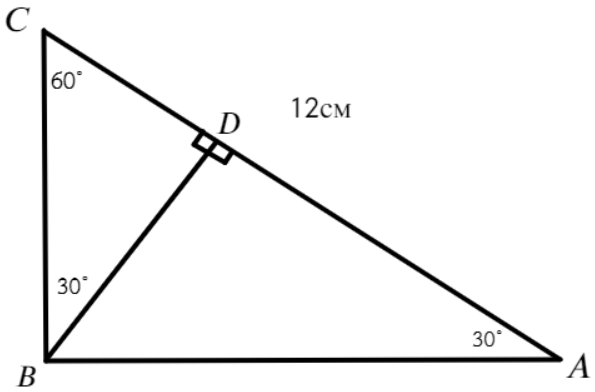
\includegraphics[scale=0.35]{g22.png}}
\end{figure}\\
$\angle C=90^\circ-\angle A=90^\circ-30^\circ=60^\circ,\ \angle CBD=90^\circ-\angle C=90^\circ-60^\circ=30^\circ.$ В прямоугольном треугольнике $ABC$ катет $BC$ лежит напротив угла в $30^\circ,$ а значит $BC=AC:2=12:2=6$см. В прямоугольном треугольнике $BCD$ катет $CD$ лежит напротив угла в $30^\circ,$ а значит $CD=BC:2=6:2=3$см. Тогда $DA=AC-CD=12-3=9$см.\\
23. Для стороны есть 2 варианта: она может быть боковой стороной или основанием. Для угла также есть 2 варианта: он может быть углом при вершине или при основание. Таким образом, существует $2\cdot2=4$ неравных между собой треугольников.\\
24. Если у равнобедренного треугольника один из углов равен $60^\circ,$ остальные его углы тоже равны $60^\circ,$ а значит он является равносторонним. Так как длина стороны задана, такой треугольник существует только один.\\
25. \begin{figure}[ht!]
\center{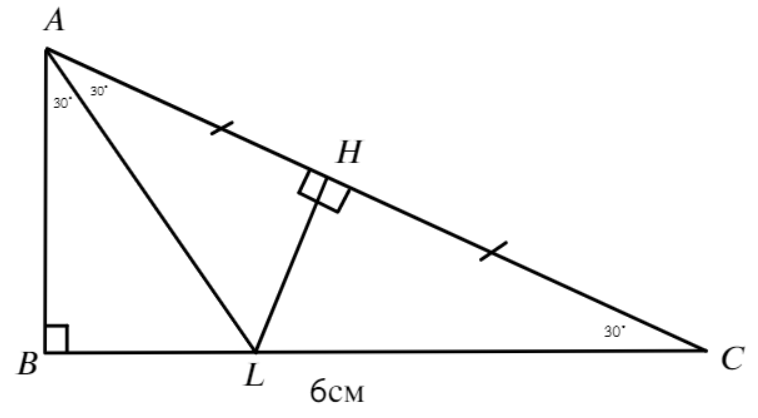
\includegraphics[scale=0.35]{g25.png}}
\end{figure}\\
Так как $AL$ является биссектрисой, $\angle BAL=\angle LAC=60^\circ:2=30^\circ.$ Угол $C$ также равен $90^\circ-\angle A=90^\circ-60^\circ=30^\circ.$ В прямоугольных треугольниках $LAH$ и $LCH$ катет $LH$ лежит напротив угла в $30^\circ,$ а значит $AL=LC=2LH.$ В прямоугольном треугольнике $ABL$ катет $BL$ лежит напротив угла
в $30^\circ,$ а значит $BL=AL:2=2LH:2=LH.$ Таким образом, $BC=BL+LC=LH+2LH=3LH=6$см, откуда $LH=6:3=2$см.\newpage\noindent
26. \begin{figure}[ht!]
\center{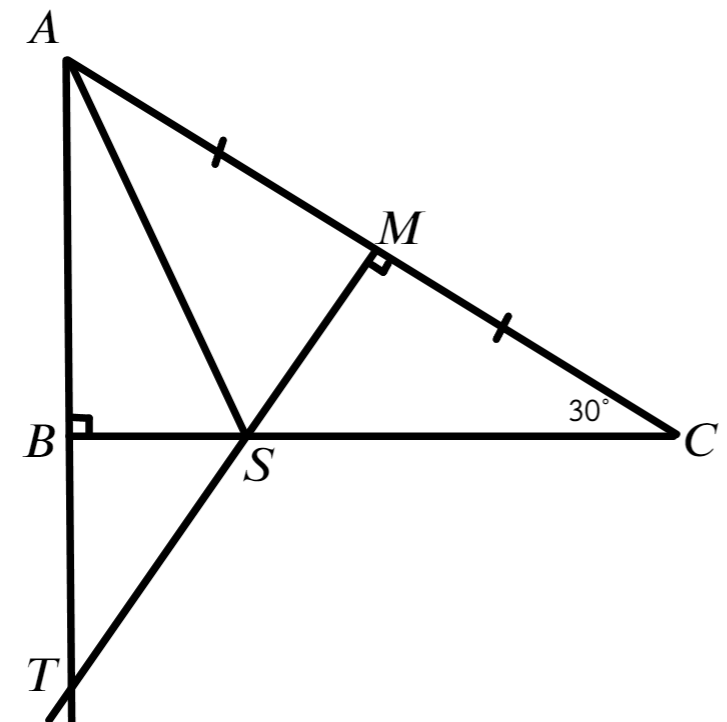
\includegraphics[scale=0.35]{g26.png}}
\end{figure}\\
$\angle C=90^\circ-\angle A=90^\circ-60^\circ=30^\circ.$ Пусть $MT$ пересекает сторону $BC$ в точке $S.$ Так как в треугольнике $ASC$ высота совпала с медианой, он является равнобедренным, поэтому $\angle SAC=\angle C=30^\circ.$ Тогда $\angle BAS=\angle A-\angle SAC=60^\circ-30^\circ=30^\circ.$ В прямоугольных треугольниках $SAM$ и $SCM$ катет $MS$ лежит напротив угла в $30^\circ,$ а значит $AS=SC=2MS.$ В прямоугольном треугольнике $ABS$ катет $BS$ лежит напротив угла
в $30^\circ,$ а значит $BS=AS:2=2MS:2=MS.$ Таким образом, $BC=BS+SC=MS+2MS=3MS=3$см, откуда $MS=3:3=1$см. Из треугольника $TAM$ найдём $\angle ATM=90^\circ-60^\circ=30^\circ.$ В прямоугольном треугольнике $TBS$ катет $BS$ лежит напротив угла в $30^\circ,$ значит $ST=2BS=2\cdot1=2$см. Таким образом, $MT=MS+ST=1+2=3$см.\\
27. \begin{figure}[ht!]
\center{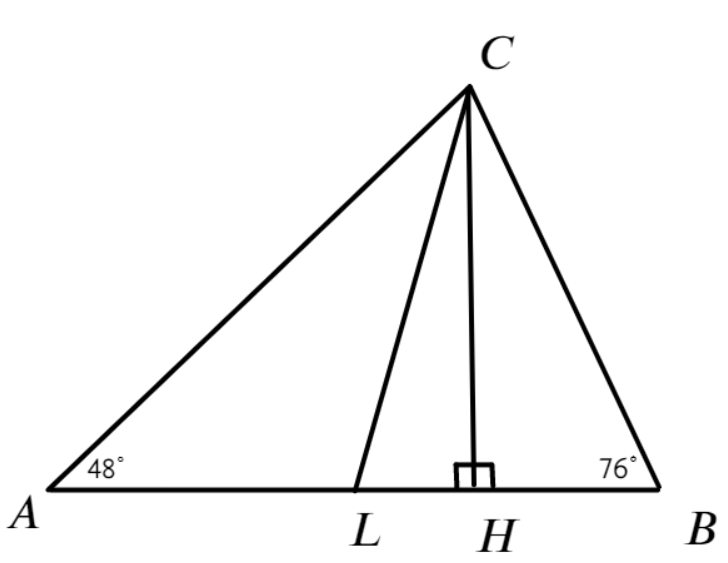
\includegraphics[scale=0.35]{g27.png}}
\end{figure}\\
$\angle C=180^\circ-\angle A-\angle B=180^\circ-48^\circ-76^\circ=56^\circ.$ Пусть $CH$ высота, а $CL$ --- биссектриса. Тогда $\angle BCH=90^\circ-76^\circ=14^\circ,$ а $\angle BCL=56^\circ:2=28^\circ.$ Таким образом, $\angle LCH=\angle BCL- \angle BCH=28^\circ-14^\circ=14^\circ.$\\
28. \begin{figure}[ht!]
\center{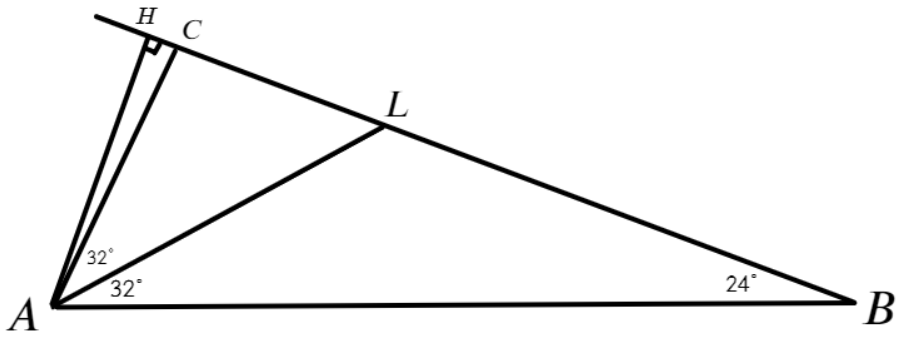
\includegraphics[scale=0.35]{g28.png}}
\end{figure}\\
$\angle C=180^\circ-\angle A-\angle B=180^\circ-64^\circ-24^\circ=92^\circ.$ Так как $\angle C>90^\circ,$ высота из точки $A$ падает на продолжение стороны $BC.$   Пусть $AH$ высота, а $AL$ --- биссектриса. Тогда $\angle CAH=90^\circ-\angle HCA=90^\circ-(180^\circ-\angle C)=90^\circ-88^\circ=2^\circ,$ а $\angle CAL=64^\circ:2=32^\circ.$ Таким образом, $\angle LAH=\angle CAL+ \angle CAH=32^\circ+2^\circ=34^\circ.$\newpage\noindent
29. \begin{figure}[ht!]
\center{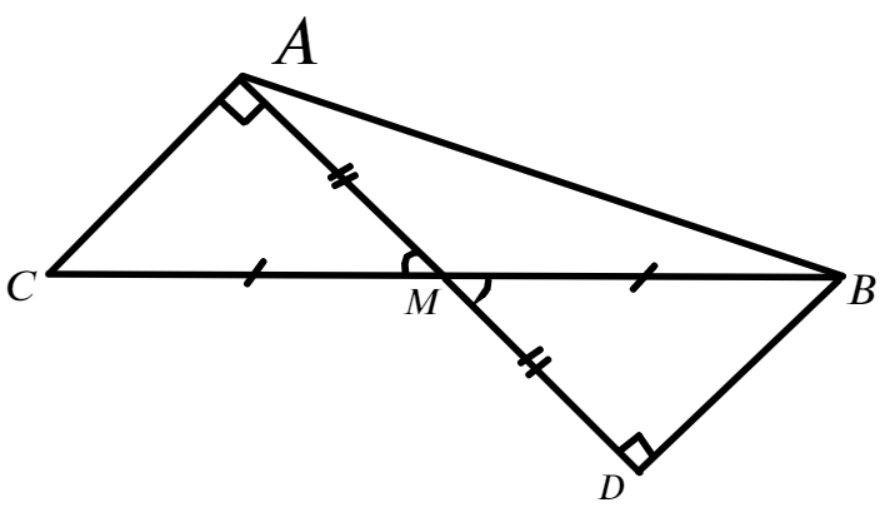
\includegraphics[scale=0.35]{g29.png}}
\end{figure}\\
Сделаем стандартное дополнительное построение: продлим медиану $AM$ на свою длину: $AM=MD.$ Тогда $\left.\begin{array}{l}AM=MD\text{ по построению},\\
 CM=MB\text{ ($AM$ --- медиана)},\\ \angle BMD=\angle CMA\text{ (вертикальные).}\end{array}\right\}\Rightarrow
\Delta BMD=\Delta CMA\text{ по I признаку}\Rightarrow AC=BD$ и $\angle BDM=\angle CAM=90^\circ.$ Треугольник $BAD$ является прямоугольным и в нём $AB=2AC=2BD,$ значит катет $BD$ лежит напротив угла в $30^\circ,$ поэтому $\angle BAM=30^\circ.$ Таким образом, $\angle BAC=90^\circ+30^\circ=120^\circ.$\\
30. \begin{figure}[ht!]
\center{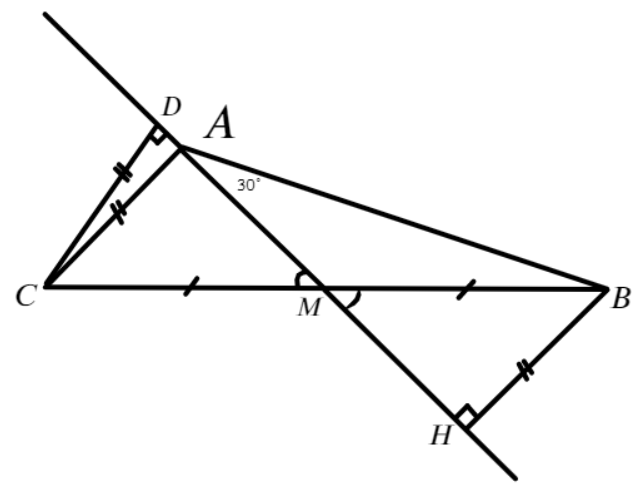
\includegraphics[scale=0.35]{g30.png}}
\end{figure}\\
Сделаем дополнительное построение: опустим из точки $B$ перпендикуляр $BH$ на продолжение медианы $AM.$ Треугольник $ABH$ является прямоугольным и катет $BH$ лежит напротив угла в $30^\circ,$ поэтому $BH=\frac{1}{2}AB=AC.$ Теперь опустим перпендикуляр $CD$ из точки $C$ на прямую $AM.$ Углы $DMC$ и $HMB$ являются вертикальными, $CM=MB$ (так как $AM$ медиана), значит прямоугольные треугольники $DMC$ и $HMB$ равны по гипотенузе и острому углу, поэтому $CD=BH=AC.$ Но тогда в прямоугольном треугольнике $CDA$ катет равен гипотенузе, что невозможно, значит точка $D$ совпадает с точкой $A$ и $\angle CAM=90^\circ.$ Таким образом, $\angle BAC=90^\circ+30^\circ=120^\circ.$\newpage
\noindent31. \begin{figure}[ht!]
\center{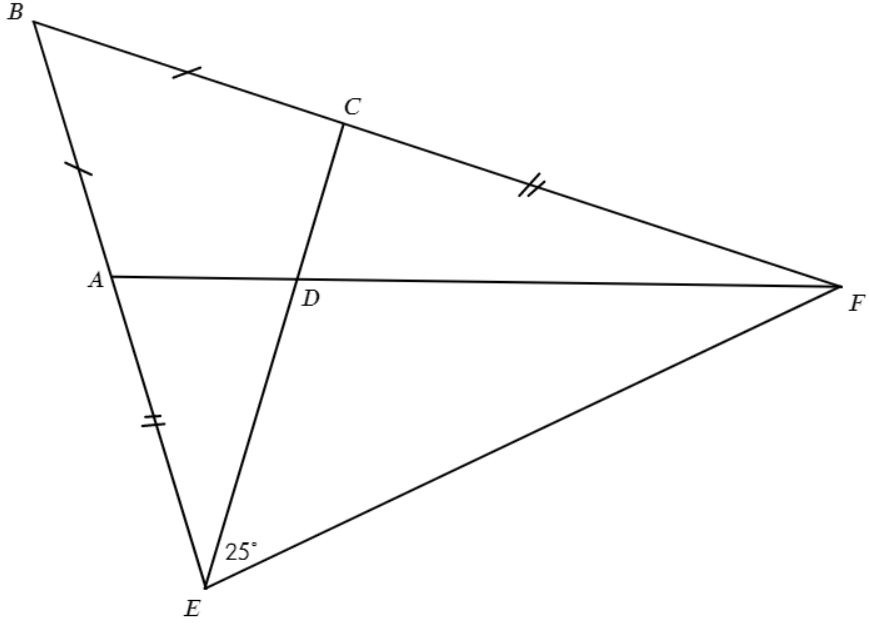
\includegraphics[scale=0.35]{g31.png}}
\end{figure}\\
Заметим, что $AE=BE-AB=BF-BC=CF.$ Треугольник $EBF$ является равнобедренным $(BE=BF),$ значит $\angle BEF=\angle BFE.$ Тогда
$\left.\begin{array}{l}AE=CF,\\
\angle AEF=\angle CFE,\\
EF\text{--- общая.}  \end{array}\right\}\Rightarrow \Delta AEF=\Delta CFE\text{ по I призн.}$\\$\Rightarrow \angle EFD=\angle EFA=\angle CEF=\angle DEF=25^\circ.$\\
32. \begin{figure}[ht!]
\center{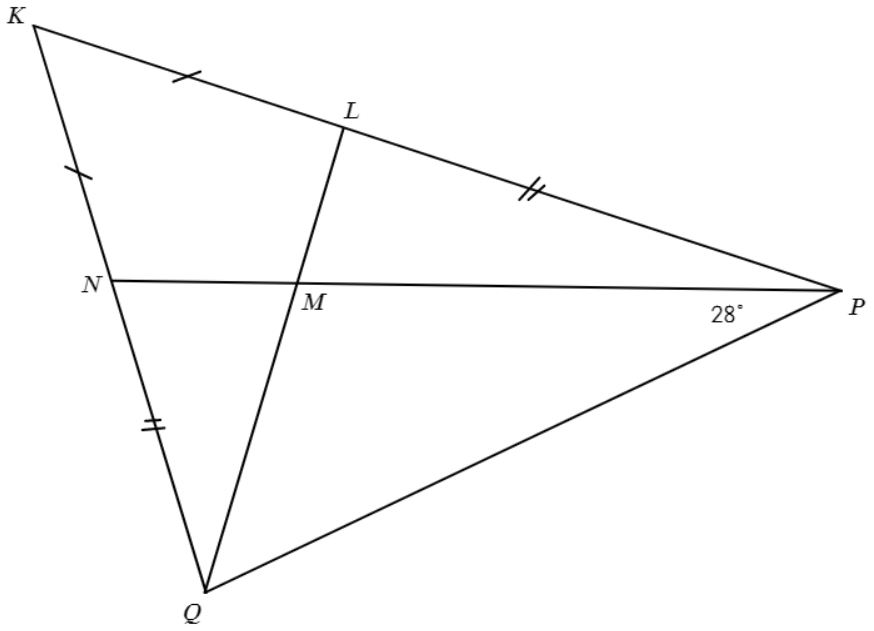
\includegraphics[scale=0.35]{g32.png}}
\end{figure}\\
Заметим, что $NQ=KQ-KN=KP-KL=LP.$ Треугольник $QKP$ является равнобедренным $(KQ=KP),$ значит $\angle KPQ=\angle KQP.$ Тогда
$\left.\begin{array}{l}NQ=LP,\\
\angle NQP=\angle LPQ,\\
QP\text{--- общая.}  \end{array}\right\}\Rightarrow \Delta QNP=\Delta PLQ\text{ по I призн.}$\\$\Rightarrow \angle PQM=\angle PQL=\angle NPQ=\angle MPQ=28^\circ.$\\
33. \begin{figure}[ht!]
\center{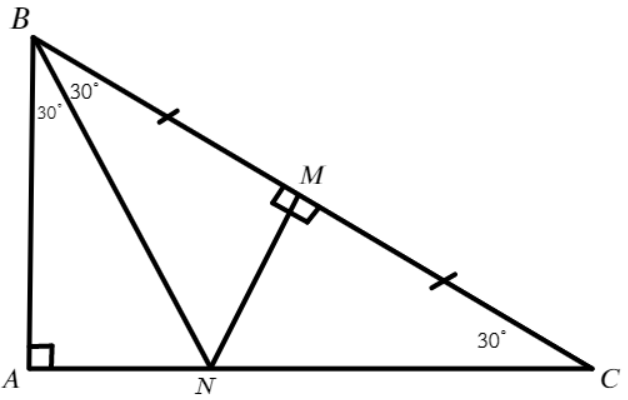
\includegraphics[scale=0.35]{g33.png}}
\end{figure}\\
Пусть $\angle C=30^\circ.$ В треугольнике $NBC$ высота $NM$ совпадает с медианой, значит он равнобедренный и $BN=NC,\ \angle NBC=\angle NCB=30^\circ.$ Тогда $\angle ABN=180^\circ-90^\circ-30^\circ-30^\circ=30^\circ.$ По теореме о катете, лежащем напротив угла в $30^\circ,$ для треугольников $ABN,\ MBN$ и $NMC$ имеем $NC=2NM,\ AN=\frac{1}{2}BN=NM,$ откуда $AC=AN+NC=NM+2NM=3NM,$ ч.т.д.\newpage
\noindent34. \begin{figure}[ht!]
\center{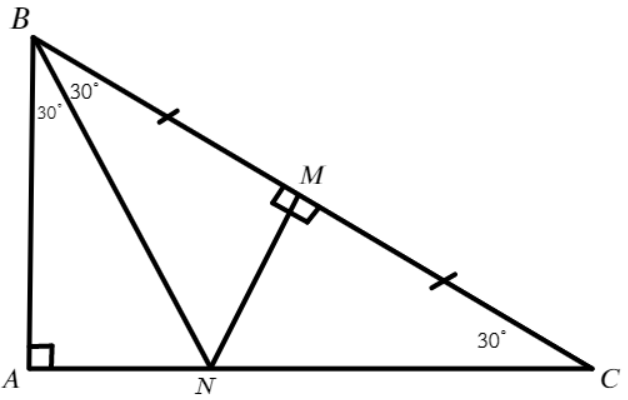
\includegraphics[scale=0.35]{g33.png}}
\end{figure}\\
Пусть $\angle B=60^\circ,$ тогда $\angle C=90^\circ-60^\circ=30^\circ.$ В треугольнике $NBC$ высота $NM$ совпадает с медианой, значит он равнобедренный и $BN=NC,\ \angle NBC=\angle NCB=30^\circ.$ Тогда $\angle ABN=180^\circ-90^\circ-30^\circ-30^\circ=30^\circ.$ По теореме о катете, лежащем напротив угла в $30^\circ,$ для треугольников $ABN,\ MBN$ и $NMC$ имеем $NC=2NM,\ AN=\frac{1}{2}BN=NM,$ откуда $AC=AN+NC=NM+2NM=3NM,$ ч.т.д.\\
35. Если внешний угол равен $130^\circ,$ внутренний угол равен $180^\circ-130^\circ=50^\circ.$ Если это угол при вершине, два других угла равны $(180^\circ-50^\circ):2=65^\circ.$ Если это угол при основании, то угол при вершине равен $180^\circ-2\cdot50^\circ=80^\circ.$ Таким образом, треугольник может иметь углы  $50^\circ,\ 50^\circ,\ 80^\circ$ или $50^\circ,\ 65^\circ,\ 65^\circ.$\\
36. Третья сторона треугольника может быть равна 6см или 10см. Для обоих случаев выполняется неравенство треугольника $(6+6>10,\ 6+10>10),$ значит периметр может быть равен $2\cdot6+10=22$см или $2\cdot10+6=26$см.\\
37. \begin{figure}[ht!]
\center{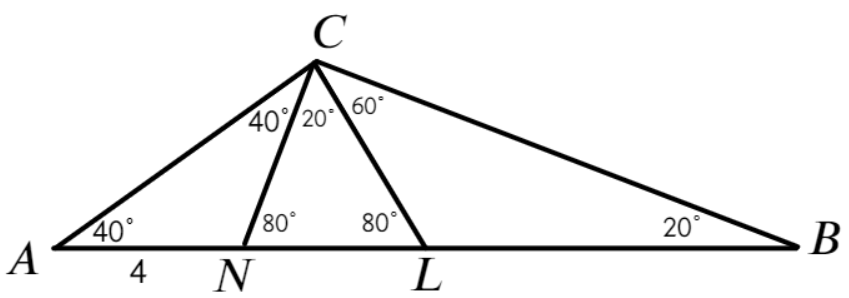
\includegraphics[scale=0.35]{g37.png}}
\end{figure}\\
Пусть $CL$ --- биссектриса. Сделаем дополнительное построение: отметим на стороне $AB$ точку $N$ так, чтобы $BC=BN.$ Тогда $AN=AB-BN=AB-BC=4.$ Треугольник $CBN$ является равнобедренным с углом при вершине $20^\circ,$ значит $\angle CNB=\angle NCB=(180^\circ-20^\circ):2=80^\circ.$ Угол $C$ равен $180^\circ-20^\circ-40^\circ=120^\circ,$ значит $\angle LCB=120^\circ:2=60^\circ,\ \angle NCL=80^\circ-60^\circ=20^\circ,\ \angle ACN=60^\circ-20^\circ=40^\circ,\ \angle CLN=180^\circ-20^\circ-80^\circ=80^\circ.$ Таким образом, треугольники $ACN$ и $NCL$ являются равнобедренными, а поэтому $CL=CN=AN=4.$\\
38. \begin{figure}[ht!]
\center{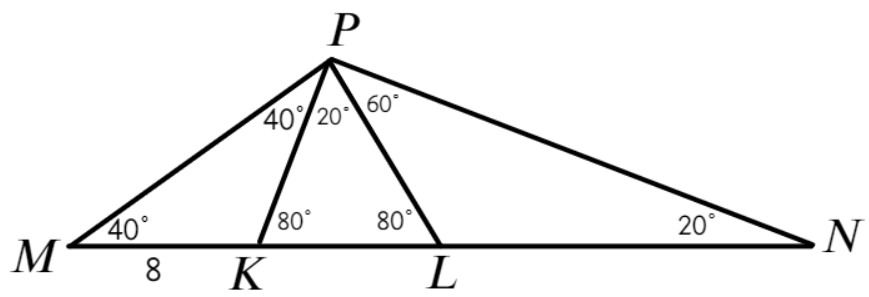
\includegraphics[scale=0.35]{g38.png}}
\end{figure}\\
Пусть $PL$ --- биссектриса. Сделаем дополнительное построение: отметим на стороне $MN$ точку $K$ так, чтобы $NP=NK.$ Тогда $MK=MN-NK=MN-NP=8.$ Треугольник $PNK$ является равнобедренным с углом при вершине $20^\circ,$ значит $\angle PKN=\angle KPN=(180^\circ-20^\circ):2=80^\circ.$ Угол $P$ равен $180^\circ-20^\circ-40^\circ=120^\circ,$ значит $\angle LPN=120^\circ:2=60^\circ,\ \angle KPL=80^\circ-60^\circ=20^\circ,\ \angle MPK=60^\circ-20^\circ=40^\circ,\ \angle PLK=180^\circ-20^\circ-80^\circ=80^\circ.$ Таким образом, треугольники $MPK$ и $KPL$ являются равнобедренными, а поэтому $PL=PK=MK=8.$\newpage
\noindent39. \begin{figure}[ht!]
\center{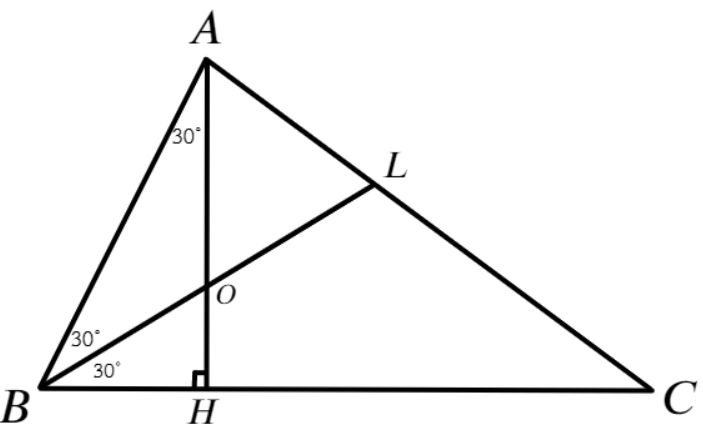
\includegraphics[scale=0.35]{g39.png}}
\end{figure}\\
Пусть $BL$ и $AH$ пересекаются в точке $O.$ Так как $BL$ является биссектрисой, $\angle OBH=\angle OBA=30^\circ.$ Из треугольника $ABH:\ \angle BAH=180^\circ-90^\circ-60^\circ=30^\circ.$ В прямоугольном треугольнике $OBH$ катет $BH$ лежит напротив угла в $30^\circ,$ поэтому $OB=2OH.$ В треугольнике $OBA$ равны углы при стороне $AB,$ значит он является равнобедренным и $AO=OB.$ Таким образом, $AO:OH=OB:OH=2OH:OH=2:1.$\\
40. \begin{figure}[ht!]
\center{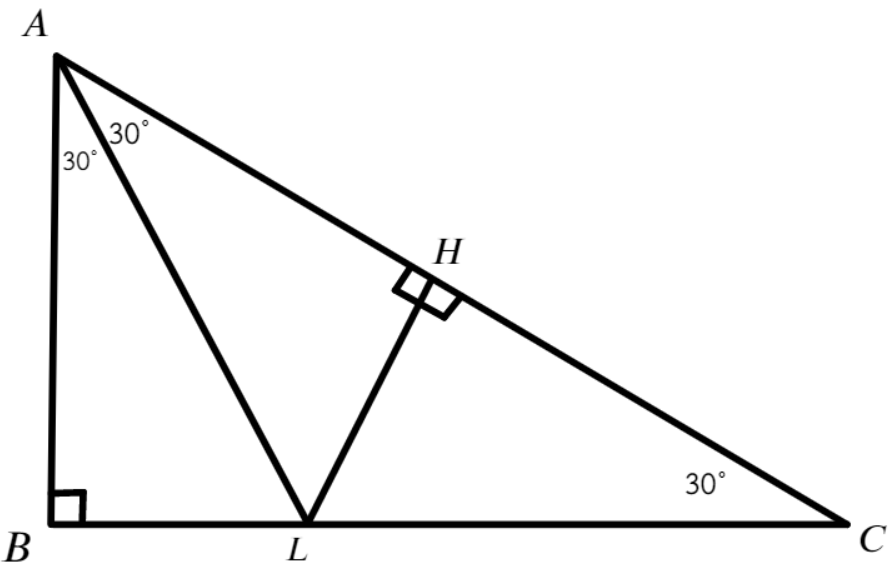
\includegraphics[scale=0.35]{g40.png}}
\end{figure}\\
Угол $B$ равен $180^\circ-90^\circ-60^\circ=30^\circ.$ Так как $AL$ является биссектрисой, $\angle BAL= \angle LAH=60^\circ:2=30^\circ.$ Тогда по теорема о катете, лежащем напротив угла в $30^\circ,$ для треугольников $LCH,\ LAH$ и $ABL$ имеем $AL=LC=2LH,\ BL=\frac{1}{2}AL=LH.$ Тогда $BC=BL+LC=LH+2LH=3LH.$ Таким образом, $LH=BC:3=6:3=2$см.\\
41. \begin{figure}[ht!]
\center{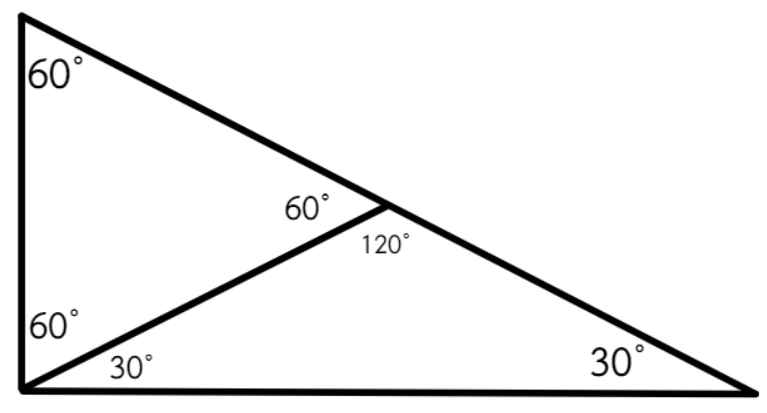
\includegraphics[scale=0.35]{g41.png}}
\end{figure}\\
Да, пример изображён на картинке.\\
42. \begin{figure}[ht!]
\center{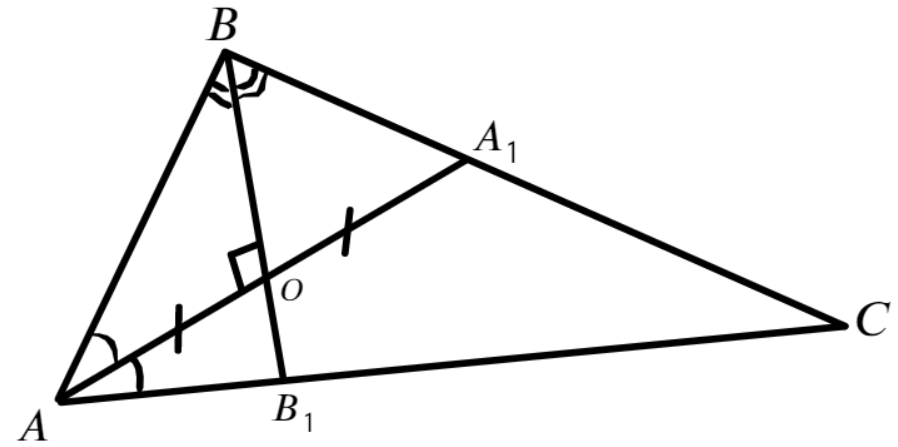
\includegraphics[scale=0.35]{g42.png}}
\end{figure}\\
Пусть биссектриса $BB_1$ поделила биссектрису $AA_1$ пополам. Тогда в треугольнике $ABA_1$ биссектриса $BO$ является медианой, а значит он равнобедренный и она является также и высотой. Но тогда $\angle BAO+\angle ABO=90^\circ\Rightarrow \angle A+\angle B=180^\circ,$ что невозможно.\\
43. \begin{figure}[ht!]
\center{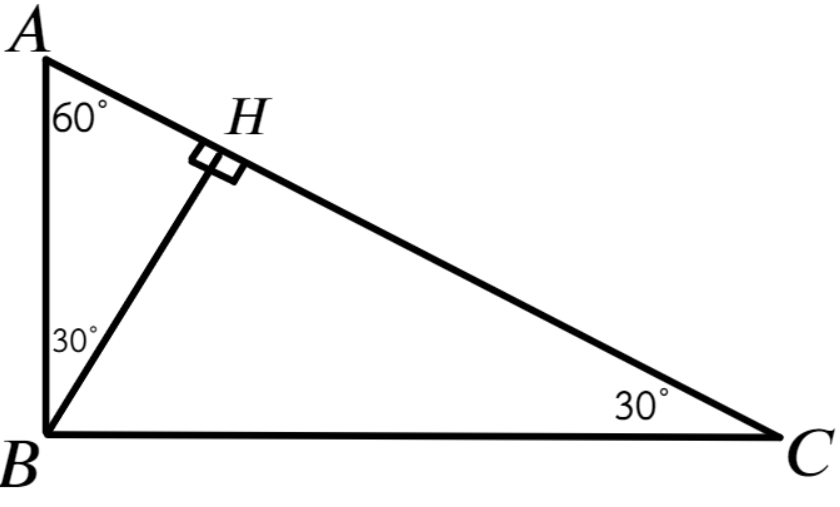
\includegraphics[scale=0.35]{g43.png}}
\end{figure}\\
Пусть $\angle C=30^\circ,$ тогда $\angle A=90^\circ-30^\circ=60^\circ,\ \angle ABH=90^\circ-60^\circ=30^\circ.$ По теореме о катете, лежащем напротив угла в $30^\circ,$ для треугольников $ABH$ и $ABC$ имеем $AB=2AH,\ AC=2AB=4AH.$ Значит, $AH=AC:4=4:4=1$см, а $HC=AC-AH=4-1=3$см.\\
44. \begin{figure}[ht!]
\center{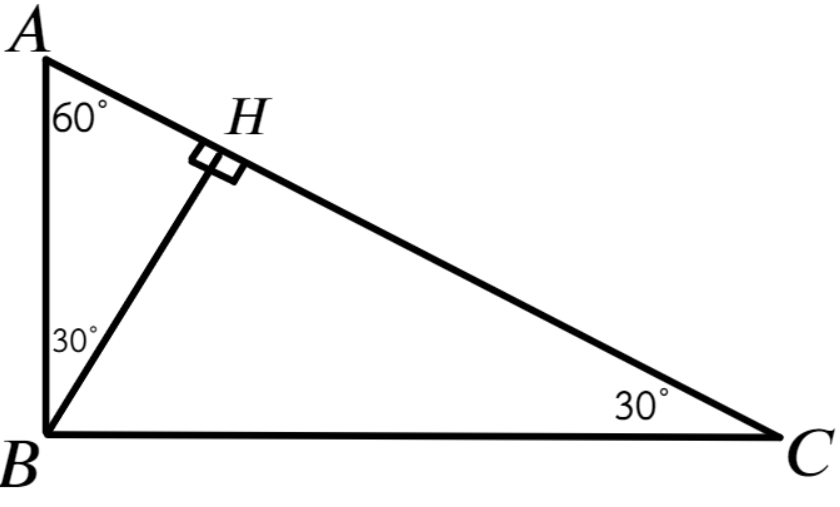
\includegraphics[scale=0.35]{g43.png}}
\end{figure}\\
Пусть $\angle C=30^\circ,$ тогда $\angle A=90^\circ-30^\circ=60^\circ,\ \angle ABH=90^\circ-60^\circ=30^\circ.$ По теореме о катете, лежащем напротив угла в $30^\circ,$ для треугольников $ABH$ и $ABC$ имеем $AB=2AH,\ AC=2AB=4AH.$ Значит, $AH=AC:4=6:4=1,5$см, а $HC=AC-AH=6-1,5=4,5$см.\\
45. \begin{figure}[ht!]
\center{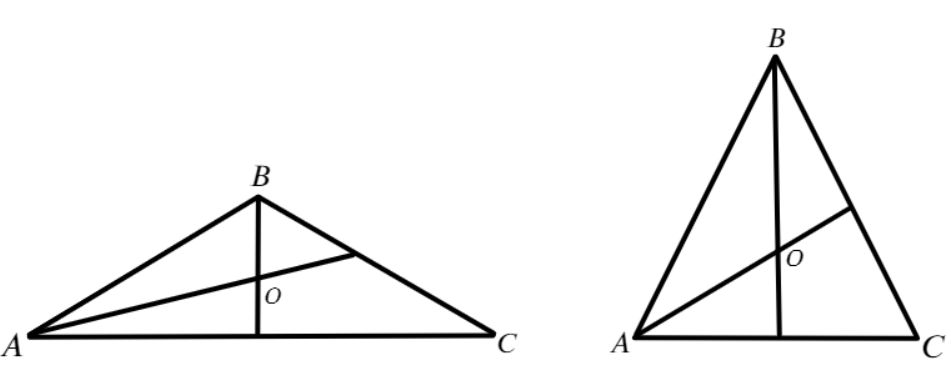
\includegraphics[scale=0.35]{g45.png}}
\end{figure}\\
Возможны два случая: в треугольнике угол при вершине равен $5x,$ а углы при основании по $2x$ и наоборот, угол при вершине равен $2x,$ а углы при основании --- по $5x.$ В первом случае $5x+2\cdot2x=180^\circ,\ 9x=180^\circ,\ x=20^\circ,$ значит угол при вершине равен $5\cdot20^\circ=100^\circ,$ а углы при основании равны $2\cdot20^\circ=40^\circ.$ Тогда $\angle AOB=180^\circ-\frac{1}{2}\angle A-\frac{1}{2}\angle B=180^\circ-20^\circ-50^\circ=110^\circ.$ Так как углом между прямыми является наименьший из углов, образованных этими прямыми, угол между биссектрисами в этом случае равен $180^\circ-110^\circ=70^\circ.$ Во втором случае $2x+2\cdot5x=180^\circ,\ 12x=180^\circ,\ x=15^\circ,$ значит угол при вершине равен $2\cdot15^\circ=30^\circ,$ а углы при основании равны $5\cdot15^\circ=75^\circ.$
Тогда $\angle AOB=180^\circ-\frac{1}{2}\angle A-\frac{1}{2}\angle B=180^\circ-15^\circ-37^\circ30'=127^\circ30'.$ Так как углом между прямыми является наименьший из углов, образованных этими прямыми, угол между биссектрисами в этом случае равен $180^\circ-127^\circ30'=52^\circ30'.$\newpage
\noindent46. \begin{figure}[ht!]
\center{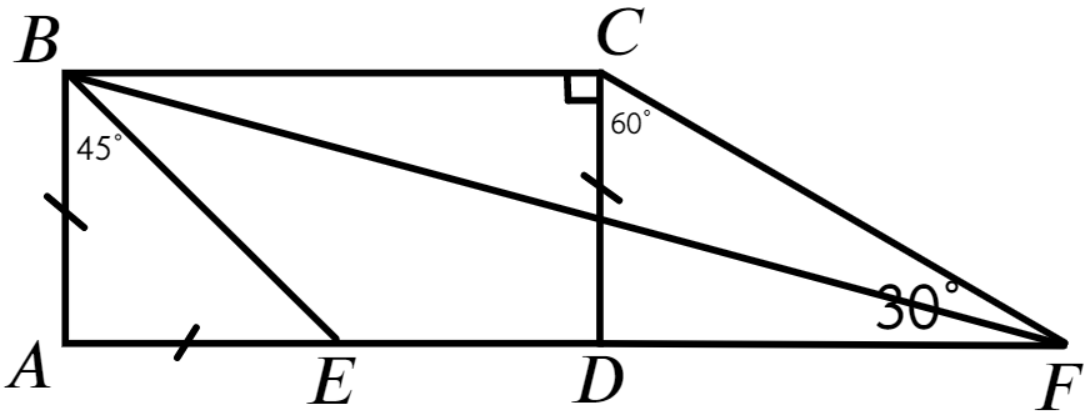
\includegraphics[scale=0.35]{g46.png}}
\end{figure}\\
Так как $AE=\frac{1}{2}AD=\frac{1}{2}BC=AB,$ треугольник $ABE$ является равнобедренным и поэтому $\angle ABE=(180^\circ-90^\circ):2=45^\circ.$ В прямоугольном треугольнике $CDF$ угол $DCF$ равен $90^\circ-30^\circ=60^\circ$ и катет $CD$ лежит напротив угла в $30^\circ,$ поэтому $CF=2CD=2AB=BC.$ Тогда треугольник $BCF$ является равнобедренным и угол при его вершине $C$ равен $90^\circ+60^\circ=150^\circ,$ а поэтому $\angle FBC=(180^\circ-150^\circ):2=15^\circ.$ Таким образом, $\angle EBF=90^\circ-45^\circ-15^\circ=30^\circ.$\\
47. \begin{figure}[ht!]
\center{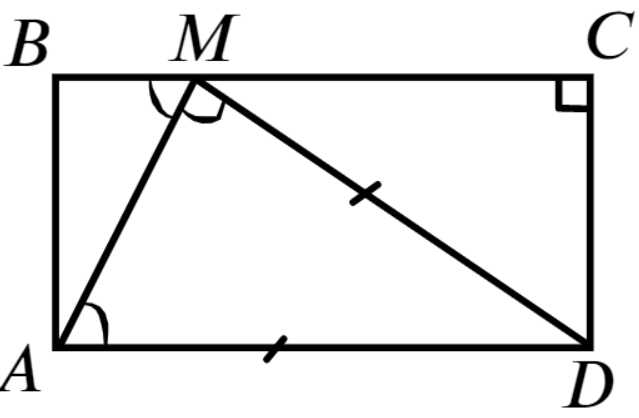
\includegraphics[scale=0.35]{g47.png}}
\end{figure}\\
Углы $BMA$ и $MAD$ являются накрест лежащими при параллельных прямых $BC$ и $AD,$ поэтому $\angle MAD=\angle BMA=\angle AMD$ (т.к. $MA$ --- биссектриса). Тогда в треугольнике $AMD$ равны углы при стороне $AM,$ значит он является равнобедренным и $MD=AD=2AB=2CD.$ Таким образом, в прямоугольном треугольнике $MCD$ катет $CD$ равен половине гипотенузы $MD,$ а значит он лежит напротив угла в $30^\circ,$ то есть $\angle DMC=30^\circ.$ Значит, $\angle BMA=(180^\circ-30^\circ):2=75^\circ.$\\
48. \begin{figure}[ht!]
\center{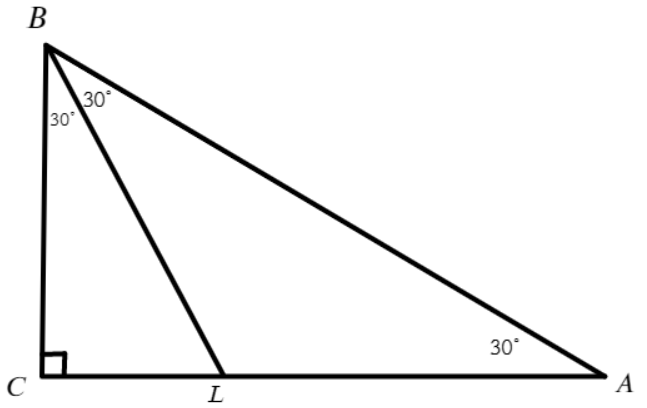
\includegraphics[scale=0.35]{g48.png}}
\end{figure}\\
Если внешний угол при вершине $B$ равен $120^\circ,$ то $\angle B=180^\circ-120^\circ=60^\circ.$ Тогда $\angle A=90^\circ-60^\circ=30^\circ$ и $\angle CBL=\angle LBA=30^\circ$ (так как $BL$ --- биссектриса). В прямоугольном треугольнике $CBL$ катет $CL$ лежит напротив угла в $30^\circ,$ поэтому $CL=\frac{1}{2}BL=\frac{1}{2}\cdot2=1$см. В треугольнике $LBA$ углы при стороне $BA$ равны, значит он равнобедренный и $AL=BL=2$см. Таким образом, $AC=CL+AL=1+2=3$см.\\
49. \begin{figure}[ht!]
\center{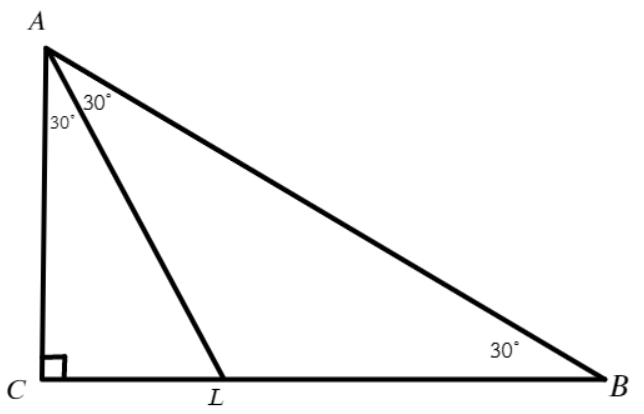
\includegraphics[scale=0.35]{g49.png}}
\end{figure}\\
Если внешний угол при вершине $B$ равен $150^\circ,$ то $\angle B=180^\circ-150^\circ=30^\circ.$ Тогда $\angle A=90^\circ-30^\circ=60^\circ$ и $\angle CAL=\angle LAB=30^\circ$ (так как $AL$ --- биссектриса). В прямоугольном треугольнике $CAL$ катет $CL$ лежит напротив угла в $30^\circ,$ поэтому $CL=\frac{1}{2}AL=\frac{1}{2}\cdot3=1,5$см. В треугольнике $LBA$ углы при стороне $BA$ равны, значит он равнобедренный и $BL=AL=3$см. Таким образом, $BC=CL+BL=1,5+3=4,5$см.\\
50. \begin{figure}[ht!]
\center{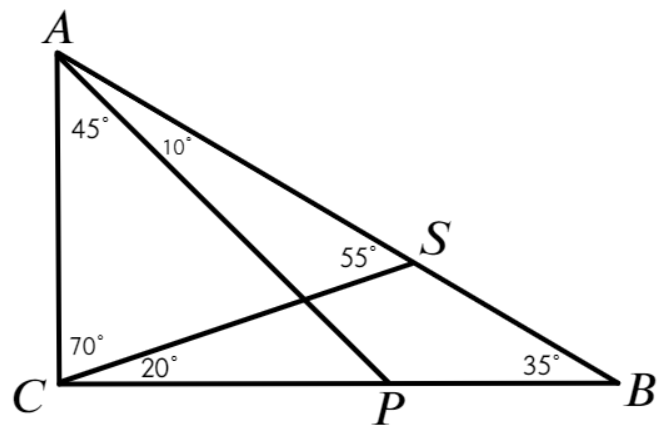
\includegraphics[scale=0.35]{g50.png}}
\end{figure}\\
Посчитаем углы на картинке: $\angle A=90^\circ-35^\circ=55^\circ,\ \angle CAP=55^\circ-10^\circ=45^\circ,\ \angle CPA=90^\circ-45^\circ=45^\circ,\ \angle CSA=20^\circ+35^\circ=55^\circ$ (как внешний в треугольнике $CSB).$ Таким образом, в треугольнике $ACP$ равны углы $CAP$ и $CPA,$ а в треугольнике $ACS$ --- углы $CAS$ и $CSA.$ Значит, эти треугольники являются равнобедренными, ч.т.д.\\
51. \begin{figure}[ht!]
\center{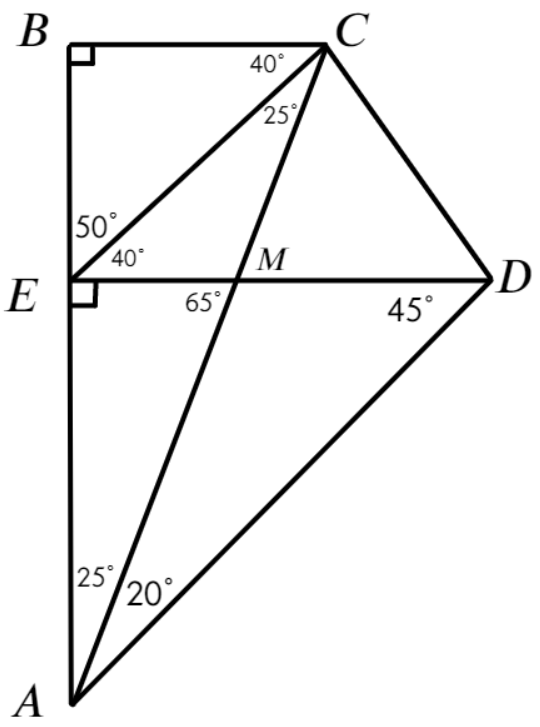
\includegraphics[scale=0.35]{g51.png}}
\end{figure}\\
Посчитаем углы на картинке: $\angle BEC=90^\circ-40^\circ=50^\circ,\ \angle CEM=90^\circ-50^\circ=40^\circ,\ \angle EAD=90^\circ-45^\circ=45^\circ,\ \angle EAC=90^\circ-65^\circ=25^\circ,\ \angle ECM=180^\circ-90^\circ-40^\circ-25^\circ=25^\circ.$ Таким образом по паре равных углов имеют треугольники $CEA$ и $EAD,$ а значит они равнобедренные и $CE=AE,\ AE=ED,$ поэтому и $CE=ED.$ Тогда треугольник $CED$ является равнобедренным, как и треугольник $CEA,$ ч.т.д.\\
52. Если меньшей стороной является основание, то стороны треугольника равны $x,\ x+8,\ x+8.$ Возможны два случая: $x+x+8=20,\ 2x=12,\ x=6$см или $x+8+x+8=20,\ 2x=4,\ x=2$см. Тогда стороны равны 6см, 14см и 14см или 2см, 10см и 10см. Неравенство треугольника выполняется для обоих случаев. Если меньшей стороной является боковая сторона, то стороны треугольника равны $x,\ x-8,\ x-8.$ Возможны два случая: $x+x-8=20,\ 2x=28,\ x=14$см или $x-8+x-8=20,\ 2x=36,\ x=18$см. Тогда стороны равны 14см, 6см и 6см или 18см, 10см и 10см. Для первого из этих случаев не выполняется неравенство треугольника: $6+6<14.$ Таким образом, длина основания может быть равна 2см, 6см или 18см.\\
53. Если меньшей стороной является основание, то стороны треугольника равны $x,\ x+6,\ x+6.$ Возможны два случая: $x+x+6=16,\ 2x=10,\ x=5$см или $x+6+x+6=16,\ 2x=4,\ x=2$см. Тогда стороны равны 5см, 11см и 11см или 2см, 8см и 8см. Неравенство треугольника выполняется для обоих случаев. Если меньшей стороной является боковая сторона, то стороны треугольника равны $x,\ x-6,\ x-6.$ Возможны два случая: $x+x-6=16,\ 2x=22,\ x=11$см или $x-6+x-6=16,\ 2x=28,\ x=14$см. Тогда стороны равны 11см, 5см и 5см или 14см, 8см и 8см. Для первого из этих случаев не выполняется неравенство треугольника: $5+5<11.$ Таким образом, длина основания может быть равна 2см, 5см или 14см.\\
54. \begin{figure}[ht!]
\center{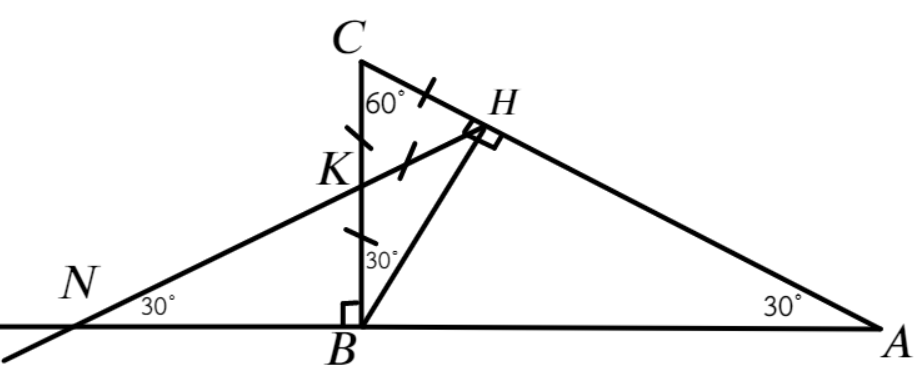
\includegraphics[scale=0.35]{g54.png}}
\end{figure}\\
Раз угол $A$ равен $30^\circ,$ угол $B$ равен $90^\circ-30^\circ=60^\circ.$ Треугольник $KCH$ является равнобедренным и один из его углов равен $60^\circ,$ значит он равносторонний и все его углы равны $60^\circ.$ Тогда $\angle NKB=\angle CKH=60^\circ$ (вертикальные), а $\angle KNB=90^\circ-60^\circ=30^\circ.$ По теореме о катете, лежащем напротив угла в $30^\circ$ для треугольников $BCH,\ KNB$ и $ABC$ имеем $CB=2CH=2KC\Rightarrow KB=CB-KC=KC,\ KN=2KB,\ AC=2CB=4KB.$ Тогда $AH=AC-CH=4KB-KB=3KB,$ а значит $AH:KN=3KB:2KB=3:2.$\\
55. \begin{figure}[ht!]
\center{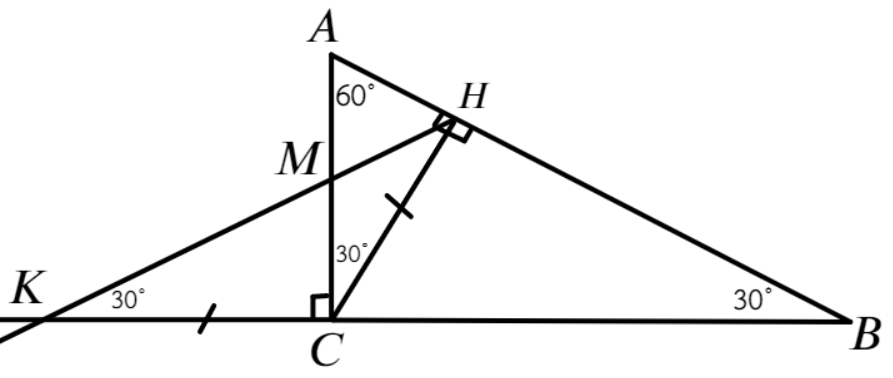
\includegraphics[scale=0.35]{g55.png}}
\end{figure}\\
Раз угол $B$ равен $30^\circ,$ угол $A$ равен $90^\circ-30^\circ=60^\circ$ и $\angle ACH=90^\circ-60^\circ=30^\circ.$  Треугольник $KHC$ является равнобедренным с углом при вершине $90^\circ+30^\circ=120^\circ$, значит $\angle KHC=\angle HKC=(180^\circ-120^\circ):2=30^\circ.$ Тогда $\angle AHM=90^\circ-30^\circ=60^\circ,$ а значит этот треугольник является равносторонним и $AH=AM=MH.$ Треугольник $MCH$ является равнобедренным, так как $\angle MCH=\angle MHC=30^\circ,$ значит $MC=MH.$  По теореме о катете, лежащем напротив угла в $30^\circ$ для треугольника $KMC$ имеем $KM=2MC.$ В треугольнике $KHB$ углы при стороне $KB$ равны по $30^\circ,$ значит он равнобедренный и  $BH=KH=KM+MH=2MC+MC=3MC.$ Таким образом, $BH:KM=3MC:2MC=3:2.$\\
56. \begin{figure}[ht!]
\center{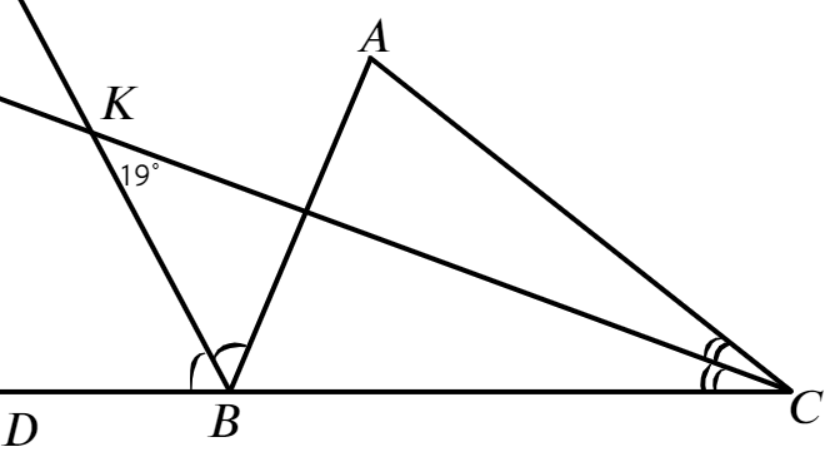
\includegraphics[scale=0.35]{g56.png}}
\end{figure}\\
Запишем сумму углов треугольника $BKC:\ 19^\circ+(180^\circ-\angle B):2+\angle B+\frac{1}{2}\angle C=180^\circ,\ \frac{1}{2}(\angle B+\angle C)=71^\circ,\ \angle B+\angle C=142^\circ.$ Тогда $\angle BAC=180^\circ-(\angle B+\angle C)=180^\circ-142^\circ=38^\circ.$\newpage
\noindent57. \begin{figure}[ht!]
\center{\includegraphics[scale=0.35]{g57.png}}
\end{figure}\\
Запишем сумму углов треугольника $ABC:\ \angle B+\angle C+52^\circ=180^\circ,\ \angle B+\angle C=128^\circ.$ Теперь запишем сумму углов треугольника $CMB:\ \angle BMC+(180^\circ-\angle C):2+\angle C+\frac{1}{2}\angle B=180^\circ,\ \angle BMC+\frac{1}{2}(\angle B+\angle C)=90^\circ,\ \angle BMC+64^\circ=90^\circ,\ \angle BMC=26^\circ.$\\
58. \begin{figure}[ht!]
\center{\includegraphics[scale=0.35]{g58.png}}
\end{figure}\\
Так как отрезки $AB$ и $CD$ равны и пересекаются в середине, $AE=BE=CE=DE.$ Так как $AD=CE=AE=DE,$ треугольник $AED$ является равносторонним, а значит $\angle AED=60^\circ=\angle BEC,$ значит треугольник $BEC$ также является равносторонним. Равные углы $BCE$ и $EDA$ являются накрест лежащими, значит прямые $BC$ и $AD$ параллельны, поэтому $\angle CBD+\angle ADB=180^\circ$ (они односторонние). $\left.\begin{array}{l}BC=AD,\\
CD=AB,\\
\angle BCD=\angle DAB  \end{array}\right\}\Rightarrow \Delta BCD=\Delta DAB\text{ по I признаку}\Rightarrow \angle CBD=\angle ADB.$ Так как $\angle CBD+\angle ADB=180^\circ,$ получаем $\angle CBD=\angle ADB=90^\circ.$ Это значит, что $MB\perp BC,$ то есть длина $BM$ и является расстоянием от точки $M$ до прямой $BC.$ Найдём $\angle EBM=90^\circ-60^\circ=30^\circ.$ Также и $\angle BEM=90^\circ-60^\circ=30^\circ.$ Поэтому треугольник $BEM$ является равнобедренным и $BM=EM.$ Теперь найдём $\angle MDE=90^\circ-60^\circ=30^\circ.$ В прямоугольном треугольнике $EMD$ катет $EM$ лежит напротив угла в $30^\circ,$ а значит $MD=2EM=2BM,$ ч.т.д.\\
59. \begin{figure}[ht!]
\center{\includegraphics[scale=0.35]{g59.png}}
\end{figure}\\
Так как отрезки $AD$ и $BC$ равны и пересекаются в середине, $AE=BE=CE=DE.$ Так как $AB=CE=AE=BE,$ треугольник $AEB$ является равносторонним, а значит $\angle AEB=60^\circ=\angle DEC,$ значит треугольник $DEC$ также является равносторонним. Равные углы $DCE$ и $EBA$ являются накрест лежащими, значит прямые $DC$ и $AB$ параллельны, поэтому $\angle CDB+\angle ABD=180^\circ$ (они односторонние). $\left.\begin{array}{l}DC=AB,\\
CB=AD,\\
\angle DCB=\angle DAB  \end{array}\right\}\Rightarrow \Delta BCD=\Delta ADB\text{ по I признаку}\Rightarrow \angle CDB=\angle ABD.$ Так как $\angle CDB+\angle ABD=180^\circ,$ получаем $\angle CDB=\angle ABD=90^\circ.$ Пусть $DH$ --- перпендикуляр, опущенный из точки $D$ на $KE$ (его длина и является искомым расстоянием). Найдём $\angle DEH=90^\circ-60^\circ=30^\circ,\ \angle EDB=90^\circ-60^\circ=30^\circ,$ тогда из треугольника $DKE:\ \angle DKE=180^\circ-90^\circ-30^\circ-30^\circ=30^\circ.$ Поэтому он является равнобедренным и $DK=DE.$ В прямоугольном треугольнике $DKH$ катет $DH$ лежит напротив угла в $30^\circ,$ значит $DK=2DH.$ Таким образом, $KC=CD+DK=ED+DK=2DK=4DH,$ ч.т.д.\\
60. \begin{figure}[ht!]
\center{\includegraphics[scale=0.35]{g60.png}}
\end{figure}\\
Обозначим $\angle BOC=x.$ Треугольник $AOC$ равнобедренный с углом при вершине $x+52^\circ,$ поэтому $\angle ACO=(180^\circ-52^\circ-x):2=64^\circ-\frac{1}{2}x.$ Треугольник $BOC$ равнобедренный с углом при вершине $x,$ поэтому $\angle OCB=(180^\circ-x):2=90^\circ-\frac{1}{2}x.$ Таким образом, $\angle ACB=90^\circ-\frac{1}{2}x-(64^\circ-\frac{1}{2}x)=26^\circ.$\\
61. \begin{figure}[ht!]
\center{\includegraphics[scale=0.35]{g61.png}}
\end{figure}\\
Обозначим $\angle BCO=x.$ Треугольник $AOC$ равнобедренный с углом при основании $x+17^\circ,$ поэтому $\angle AOC=180^\circ-2\cdot(x+17^\circ)=146^\circ-2x.$ Треугольник $BOC$ равнобедренный с углом при основании $x,$ поэтому $\angle BOC=180^\circ-2x.$ Таким образом, $\angle AOB=180^\circ-2x-(146^\circ-2x)=34^\circ.$\\
62. \begin{figure}[ht!]
\center{\includegraphics[scale=0.35]{g62.png}}
\end{figure}\\
Так как $KD\parallel AC,$ накрест лежащие углы $DCA$ и $BDC$ равны, а так как $CD$ является биссектрисой, $\angle BCD=\angle DCA=\angle BDC.$ Поэтому треугольник $BCD$ является равнобедренным и $BC=BD=KB,$ значит равнобедренным является и треугольник $KBC.$ Обозначим их углы при основании: $\angle BCD=x,\ \angle BCK=y.$ Тогда из треугольника $KCD$ имеем $2x+2y=180^\circ,\ x+y=90^\circ=\angle KCD,$ ч.т.д.\newpage\noindent
63. \begin{figure}[ht!]
\center{\includegraphics[scale=0.35]{g63.png}}
\end{figure}\\
Углы $KBA$ и $BAD$ являются накрест лежащими при параллельных прямых $KB$ и $AC,$ значит $\angle ABD=\angle KBA=\angle BAD.$ Поэтому треугольник $ABD$ является равнобедренным и $AD=BD,$ а значит равнобедренным является и треугольник $BDC$ (так как $AD=DC,\ BD$ --- медиана). Обозначим их углы при основании $\angle BAD=\angle ABD=x,\ \angle BCD=\angle CBD=y,$ тогда из треугольника $ABC$ имеем $2x+2y=180^\circ,\ x+y=90^\circ=\angle ABC,$ ч.т.д.\\
64. Возможны два случая расположения точек $P$ и $K$ на стороне $BC.$ В первом случае точки расположены в порядке $B,\ P,\ K,\ C.$
\begin{figure}[ht!]
\center{\includegraphics[scale=0.35]{g64-1.png}}
\end{figure}\\
Треугольники $APB$ и $AKC$ являются равнобедренными, обозначим их углы при основании буквами $x$ и $y.$ Тогда из треугольника $ABC$ имеем $2x+2y+30^\circ=180^\circ,\ x+y=75^\circ.$ Таким образом, $\angle BAC=x+y+30^\circ=75^\circ+30^\circ=105^\circ.$\\
Во втором случае точки расположены в порядке $B,\ K,\ P,\ C.$
\begin{figure}[ht!]
\center{\includegraphics[scale=0.35]{g64-2.png}}
\end{figure}\\
В этом случае обозначим $\angle BAK=x,\ \angle PAC=y,$ тогда $\angle B=x+30^\circ,\ \angle C=y+30^\circ.$ Из треугольника $ABC$ имеем $x+30^\circ+y+30^\circ+x+y+30^\circ=180^\circ,\ x+y=45^\circ.$ Таким образом, $\angle BAC=x+y+30^\circ=45^\circ+30^\circ=75^\circ.$\\
65. Возможны два случая расположения точек $A$ и $B$ на стороне $PC.$ В первом случае точки расположены в порядке $P,\ A,\ B,\ C.$
\begin{figure}[ht!]
\center{\includegraphics[scale=0.35]{g65-1.png}}
\end{figure}\\
Треугольники $PAK$ и $CBK$ являются равнобедренными, обозначим их углы при основании буквами $x$ и $y.$ Тогда из треугольника $PKC$ имеем $2x+2y+40^\circ=180^\circ,\ x+y=70^\circ.$ Таким образом, $\angle PKC=x+y+40^\circ=70^\circ+40^\circ=110^\circ.$\\
Во втором случае точки расположены в порядке $P,\ B,\ A,\ C.$
\begin{figure}[ht!]
\center{\includegraphics[scale=0.35]{g65-2.png}}
\end{figure}\\
В этом случае обозначим $\angle PKB=x,\ \angle AKC=y,$ тогда $\angle P=x+40^\circ,\ \angle C=y+40^\circ.$ Из треугольника $PKC$ имеем $x+40^\circ+y+40^\circ+x+y+40^\circ=180^\circ,\ x+y=30^\circ.$ Таким образом, $\angle PKC=x+y+40^\circ=30^\circ+40^\circ=70^\circ.$\\
66. \begin{figure}[ht!]
\center{\includegraphics[scale=0.35]{g66.png}}
\end{figure}\\
Чтобы найти расстояние от $A$ до $BC,$ проведём $AD\perp BC.$ Найдём $\angle C=180^\circ-120^\circ-30^\circ=30^\circ,\ \angle BAD=90^\circ-30^\circ=60^\circ, \angle BAH=180^\circ-120^\circ=60^\circ.$ Тогда прямоугольные треугольники $BAD$ и $BAH$ равны по гипотенузе ($AB$ --- общая) и острому углу, а значит $AD=AH.$ Обозначим $AD=x,$ тогда по теореме о катете, лежащем напротив угла в $30^\circ$ для треугольника $ADC,$ имеем $AC=2x.$ Таким образом, $HC=AH+AC=x+2x=3x=12$см, откуда $AD=x=4$см.\\
67. \begin{figure}[ht!]
\center{\includegraphics[scale=0.35]{g67.png}}
\end{figure}\\
Чтобы найти расстояние от $T$ до $PK,$ проведём $TD\perp PK.$ Найдём $\angle P=180^\circ-120^\circ-30^\circ=30^\circ,\ \angle KTD=90^\circ-30^\circ=60^\circ, \angle KTH=180^\circ-120^\circ=60^\circ.$ Тогда прямоугольные треугольники $KTD$ и $KTH$ равны по гипотенузе ($KT$ --- общая) и острому углу, а значит $TD=TH.$ Обозначим $TD=x,$ тогда по теореме о катете, лежащем напротив угла в $30^\circ$ для треугольника $TDP,$ имеем $TP=2x.$ Таким образом, $HP=TH+TP=x+2x=3x=21$см, откуда $TD=x=7$см.\\
68. \begin{figure}[ht!]
\center{\includegraphics[scale=0.35]{g68.png}}
\end{figure}\\
Возможны три разных порядка расположения сторон этого четырёхугольника. Возможность существования четырёхугольника с заданными сторонами и целой диагональю определяется только выполнением неравенств треугольника для всех образовавшихся треугольников. Самое маленькое целое значение, которое может принимать диагональ --- это значение 6 для диагонали $AC$ во втором случае. Самое большое --- значение 10 для диагонали $BD$ в третьем случае. Значение 5 ни одна диагональ принимать не может, потому что она должна образовывать треугольник со стороной 11, а даже $5+6\leqslant11.$ Значение 11 ни одна диагональ принимать не может, потому что она должна образовывать треугольник без стороны 11, а даже $6+5\leqslant11.$ Таким образом, длина диагонали может принимать только значения $6,\ 7,\ 8,\ 9,\ 10.$\\
69. \begin{figure}[ht!]
\center{\includegraphics[scale=0.35]{g69.png}}
\end{figure}\\
Обозначим $\angle BAM=4x,\ \angle CAM=7x,\ \angle BCK=4y,\ \angle ACK=7y.$ Тогда из треугольника $ABC:\ 4x+7x+4y+7y+37^\circ=180^\circ,\ 11(x+y)=143^\circ,\ x+y=13^\circ.$ Теперь запишем сумму углов треугольника $APC:\ 7x+7y+\angle APC=180^\circ,\ \angle APC=180^\circ-7(x+y)=180^\circ-7\cdot13^\circ=89^\circ.$\\
70. \begin{figure}[ht!]
\center{\includegraphics[scale=0.35]{g70.png}}
\end{figure}\\
Обозначим $\angle CAP=5x,\ \angle PAB=6x,\ \angle CBM=5y,\ \angle MBA=6y.$ Тогда из треугольника $ABC:\ 5x+6x+5y+6y+26^\circ=180^\circ,\ 11(x+y)=154^\circ,\ x+y=14^\circ.$ Теперь запишем сумму углов треугольника $AKB:\ 6x+6y+\angle AKB=180^\circ,\ \angle AKB=180^\circ-6(x+y)=180^\circ-6\cdot14^\circ=96^\circ.$\\
71. \begin{figure}[ht!]
\center{\includegraphics[scale=0.35]{g71.png}}
\end{figure}\\
Катет $BC$ лежит напротив угла в $30^\circ,$ значит $AC=2BC,$ поэтому $AM=\frac{1}{2}AC=BC=AD.$ Значит, треугольник $AMD$ является равнобедренным, а треугольник $BCM$ --- равносторонним ($BC=CM$ и $\angle C=90^\circ-\angle A=60^\circ.)$ Тогда $\angle DMA=(180^\circ-30^\circ):2=75^\circ,\ \angle PMD=180^\circ-60^\circ-75^\circ=45^\circ,\ \angle PDM=90^\circ-45^\circ=45^\circ,$ поэтому треугольник $PMD$ также является равнобедренным, $PM=PD.$ Найдём $\angle PBD=90^\circ-60^\circ=30^\circ,$ значит по теореме о катете, лежащем напротив угла в $30^\circ$ имеем $BD=2PD.$ Таким образом, $2P_{\Delta MDP}=2(PM+MD+PD)=
2PM+2MD+2PD=2PD+2PD+2MD=2BD+2MD=BD+MD+(BD+MD)>BD+MD+BM=P_{\Delta MDB},$ ч.т.д. ($BD+MD>BM$ по неравенству треугольника).\newpage
\noindent72. \begin{figure}[ht!]
\center{\includegraphics[scale=0.35]{g72.png}}
\end{figure}\\
Найдём $\angle B=90^\circ-60^\circ=30^\circ.$ Катет $AC$ лежит напротив угла в $30^\circ,$ значит $AB=2AC,$ поэтому $BD=\frac{1}{2}AB=AC=BM.$ Значит, треугольник $BMD$ является равнобедренным, а треугольник $ACD$ --- равносторонним ($AC=AD$ и $\angle A=60^\circ.)$ Тогда $\angle BDM=(180^\circ-30^\circ):2=75^\circ,\ \angle MDK=180^\circ-60^\circ-75^\circ=45^\circ,\ \angle DMK=90^\circ-45^\circ=45^\circ,$ поэтому треугольник $MDK$ также является равнобедренным, $KM=KD.$ Найдём $\angle KCM=90^\circ-60^\circ=30^\circ,$ значит по теореме о катете, лежащем напротив угла в $30^\circ$ имеем $MC=2KM.$ Таким образом, $2P_{\Delta MDK}=2(KD+MD+KM)=
2KD+2MD+2KM=2KM+2KM+2MD=2MC+2MD=MC+MD+(MC+MD)>MC+MD+CD=P_{\Delta DMC},$ ч.т.д. ($MC+MD>CD$ по неравенству треугольника).\\
73. \begin{figure}[ht!]
\center{\includegraphics[scale=0.35]{g73.png}}
\end{figure}\\
Так как $ABCD$ квадрат, а треугольник $AMB$ равносторонний, имеем $AD=BC=AB=AM=BM,$ поэтому треугольники $DAM$ и $CBM$ являются равнобедренными. Углы $DAM$ и $CBM$ равны $90^\circ+60^\circ=150^\circ,$ а значит $\angle ADM=\angle BCM=(180^\circ-150^\circ):2=15^\circ.$ Таким образом, $\angle MDC=\angle MCD-90^\circ-15^\circ=75^\circ,\ \angle DMC=180^\circ-75^\circ-75^\circ=30^\circ.$\\
74.  \begin{figure}[ht!]
\center{\includegraphics[scale=0.35]{g74.png}}
\end{figure}\\
Так как $ABCD$ квадрат, а треугольник $ANB$ равносторонний, имеем $AD=BC=AB=AN=BN,$ поэтому треугольники $DAN$ и $CBN$ являются равнобедренными. Углы при их вершинах равны $90^\circ-60^\circ=30^\circ,$ значит $\angle ADN=\angle BCN=(180^\circ-30^\circ):2=75^\circ.$ Таким образом, $\angle NDC=\angle NCD=90^\circ-75^\circ=15^\circ,\ \angle DNC=180^\circ-15^\circ-15^\circ=150^\circ.$\newpage
\noindent75. \begin{figure}[ht!]
\center{\includegraphics[scale=0.35]{g75.png}}
\end{figure}\\
Пусть $\angle C=30^\circ,$ тогда $\angle A=90^\circ-30^\circ=60^\circ,\ \angle ABH=90^\circ-60^\circ=30^\circ.$ По теореме о катете, лежащем напротив угла в $30^\circ,$ для треугольников $ABH$ и $ABC$ имеем $AB=2AH,\ AC=2AB=4AH=8,\ AH=2,\ HC=8-2=6.$\\
76. \begin{figure}[ht!]
\center{\includegraphics[scale=0.35]{g76.png}}
\end{figure}\\
Пусть $\angle A=60^\circ,$ тогда $\angle C=90^\circ-60^\circ=30^\circ,\ \angle ABH=90^\circ-60^\circ=30^\circ.$ По теореме о катете, лежащем напротив угла в $30^\circ,$ для треугольников $ABH$ и $ABC$ имеем $AB=2AH,\ AC=2AB=4AH,\ HC=4AH-AH=3AH=12,\ AH=4,\ AC=4\cdot4=16.$\\
77. \begin{figure}[ht!]
\center{\includegraphics[scale=0.35]{g77.png}}
\end{figure}\\
$\left.\begin{array}{l}AB=AD,\\
BC=CD,\\
AC\text{--- общая.}  \end{array}\right\}\Rightarrow \Delta ABC=\Delta ADC\text{ по III признаку.}$ Значит, $\angle BAC=\angle DAC$ и $AO$ является биссектрисой равнобедренного треугольника $ABD,$ а значит является и высотой, ч.т.д.\\
78. \begin{figure}[ht!]
\center{\includegraphics[scale=0.35]{g78.png}}
\end{figure}\\
В прямоугольном треугольнике $BCC_1$ катет $BC_1=8$см в 2 раза меньше гипотенузы $CC_1=16$см, значит $\angle BCC_1=30^\circ.$ Так как $CC_1$ биссектриса, $\angle C=2\cdot30^\circ=60^\circ,$ а значит $\angle A=90^\circ-60^\circ=30^\circ$ и внешний угол при вершине $A$ равен $180^\circ-30^\circ=150^\circ.$\\
79. \begin{figure}[ht!]
\center{\includegraphics[scale=0.35]{g79.png}}
\end{figure}\\
В прямоугольном треугольнике $BCD$ катет $BD$ в 2 раза меньше гипотенузы $BC,$ значит $\angle BCD=30^\circ,\ \angle B=90^\circ-30^\circ=60^\circ,\ \angle A=90^\circ-60^\circ=30^\circ.$ Тогда по теореме о катете, лежащем напротив угла в $30^\circ,$ для треугольников $BCD$ и $ABC$ имеем $BD=4:2=2,\ AB=2\cdot4=8,$ значит  $AD=8-2=6.$\\
80. В треугольнике напротив большей стороны лежит больший угол, значит наибольшим является $\angle M.$\\
81. Внутренние углы, смежные к данным внешним, равны $180^\circ-80^\circ=100^\circ$ и $180^\circ-115^\circ=65^\circ.$ Значит, третий угол равен $180^\circ-100^\circ-65^\circ=15^\circ.$\\
82. Нарисуем и подсчитаем, получается 11 частей.
\begin{figure}[ht!]
\center{\includegraphics[scale=0.35]{g82.png}}
\end{figure}\\
83. Эта сторона не может быть 4см или меньше, так как не выполняется неравенство треугольника: $2+4\leqslant6.$ Аналогично эта сторона не может быть 8см или больше, так как $2+6\leqslant8.$ Значит, она может быть равна только 5см, 6см или 7см.\\
84. \begin{figure}[ht!]
\center{\includegraphics[scale=0.35]{g84.png}}
\end{figure}\\
Найдём $\angle KMH=90^\circ-60^\circ=30^\circ,\ \angle L=90^\circ-60^\circ=30^\circ.$ По теореме о катете, лежащем напротив угла в $30^\circ,$ для треугольников $MKH$ и $KML$ имеем $KM=2\cdot6=12,\ KL=2\cdot12=24.$ Тогда $LH=KL-KH=24-6=18.$\newpage
\noindent85. \begin{figure}[ht!]
\center{\includegraphics[scale=0.35]{g85.png}}
\end{figure}\\
В прямоугольном треугольнике $BCD$ катет $DC$ в 2 раза меньше гипотенузы $BC,$ значит $\angle CBD=30^\circ,\ \angle C=90^\circ-30^\circ=60^\circ,\ \angle A=90^\circ-60^\circ=30^\circ.$ Тогда по теореме о катете, лежащем напротив угла в $30^\circ,$ для треугольников $BCD$ и $ABC$ имеем $BC=2CD,\ AC=2BC=4CD,\ AD=AC-CD=3CD.$ Значит, отношение равно $3CD:CD=3:1.$\\
86. \begin{figure}[ht!]
\center{\includegraphics[scale=0.35]{g86.png}}
\end{figure}\\
Пусть $AB$ --- данная меньшая сторона. С помощью циркуля и линейки найдём её середину $M$ (это стандартное построение). После этого проведём две окружности: с радиусом, равным второй стороне и центром в точке $A$ и с радиусом, равным медиане и центром в точке $M.$ Пусть они пересекутся в точке $C$ (если такой точки нет, то соответствующего треугольника не существует). Тогда треугольник $ABC$ --- искомый.\\
87. \begin{figure}[ht!]
\center{\includegraphics[scale=0.35]{g14.png}}
\end{figure}\\
Треугольник $ABC$ равнобедренный, поэтому $\angle A=\angle C =72^\circ.$ Так как $AP$ является биссектрисой, $\angle PAC=\angle PAB=72^\circ:2=36^\circ.$ Прямые $AB$ и $PK$ параллельны, $AP$ секущая, поэтому углы $KPA$ и $PAB$ равны как накрест лежащие, откуда $\angle KPA=36^\circ.$\\
88. \begin{figure}[ht!]
\center{\includegraphics[scale=0.35]{g88.png}}
\end{figure}\\
Обозначим $\angle CAM=\angle MAB=x,\ \angle CBM=\angle MBA=y,$ тогда из треугольника $AMB$ имеем $x+y+120^\circ=180^\circ,\ x+y=60^\circ.$ Тогда из треугольника $ABC:\ 2x+2y+\angle C=180^\circ,\ \angle C=180^\circ-2\cdot60^\circ=60^\circ.$\newpage
\noindent89. \begin{figure}[ht!]
\center{\includegraphics[scale=0.35]{g89.png}}
\end{figure}\\
Одна часть периметра равна $AB+BE,$ а другая --- $EC+8.$ Так как $BE=EC,$ отличаются они на столько же, на сколько отличаются $AB$ и 8. Значит $AB$ может быть равно 6 или 10.\\
90. \begin{figure}[ht!]
\center{\includegraphics[scale=0.35]{g90.png}}
\end{figure}\\Проведём прямую и отложим из одной точки три угла, равных $54^\circ,$ как показано на рисунке. Тогда оставшийся угол равен $180^\circ-3\cdot54^\circ=18^\circ.$ Это как раз треть от $54^\circ,$ так что остаётся только построить два угла, равных полученному, внутри одного из углов, равных $54^\circ.$\\
91. \begin{figure}[ht!]
\center{\includegraphics[scale=0.35]{g91.png}}
\end{figure}\\
Обозначим $\frac{1}{2}\angle B=y,\ \frac{1}{2}\angle C=z.$ Тогда из треугольника $AOC$ имеем $70^\circ:2+z+115^\circ=180^\circ,\ z=30^\circ.$ Значит, $\angle C=2z=60^\circ, \angle B=180^\circ-70^\circ-60^\circ=50^\circ, \angle AOB=180^\circ-70^\circ:2-50^\circ:2=120^\circ,\ \angle BOC=180^\circ-60^\circ:2-50^\circ:2=125^\circ.$\\
92. \begin{figure}[ht!]
\center{\includegraphics[scale=0.35]{g92.png}}
\end{figure}\\
Обозначим $\angle A=\angle C=x,$ тогда $\angle B=180^\circ-2x.$ Запишем сумму углов треугольника $AOB:\ 70^\circ+(180^\circ-x):2+(180^\circ-(180^\circ-2x)):2=180^\circ,\ 70^\circ +90^\circ-\frac{1}{2}x+x=180^\circ,\ \frac{1}{2}x=20^\circ,\ x=40^\circ.$ Значит углы треугольника $ABC$ равны $40^\circ,\ 40^\circ$ и $180^\circ-2\cdot40^\circ=100^\circ.$\newpage\noindent
93. \begin{figure}[ht!]
\center{\includegraphics[scale=0.35]{g93.png}}
\end{figure}\\
$5AB=AC=AB+BC=AB+8,\ 4AB=8,\ AB=2.\ 4DC=BC=8,\ DC=2.$ Тогда$AD=AB+BD=AD+BC-DC=2+8-2=8.$\\
94. \begin{figure}[ht!]
\center{\includegraphics[scale=0.35]{g94.png}}
\end{figure}\\
Сумма углов невыпуклого четырёхугольника также равна $360^\circ,$ поэтому $\angle BDC=360^\circ-127^\circ-25^\circ-19^\circ=189^\circ.$ Тогда $\angle PDC=189^\circ-180^\circ=9^\circ.$\\
95. \begin{figure}[ht!]
\center{\includegraphics[scale=0.35]{g95.png}}
\end{figure}\\
$\left.\begin{array}{l}BP=AH,\\
AB\text{ --- общая.} \end{array}\right\}\Rightarrow \Delta BPA=\Delta AHB\text{ по катету и гипотенузе}\Rightarrow \angle HAB=\angle ABP=\angle CAH.$ Тогда из треугольника $APB$ имеем $\angle CAH=90^\circ:3=30^\circ,$ тогда $\angle C=\angle B=\angle A=60^\circ.$\\
96. \begin{figure}[ht!]
\center{\includegraphics[scale=0.35]{g96.png}}
\end{figure}\\
Пусть $\angle A=3x,\ \angle B=5x,\ \angle C=2x,$ тогда $3x+5x+2x=180^\circ,\ 10x=180^\circ,\ x=18^\circ.$ Тогда $\angle A=3\cdot18^\circ=54^\circ.$
$\left.\begin{array}{l}CM=MK,\\
BM=MA,\\
\angle CMA=\angle BMK\text{ (вертикальные).}\end{array}\right\}\Rightarrow \Delta CMA=\Delta KMB\text{ по I признаку}\Rightarrow \angle ABK=\angle MBK=\angle A=54^\circ.$\newpage
\noindent97. \begin{figure}[ht!]
\center{\includegraphics[scale=0.35]{g97.png}}
\end{figure}\\
Пусть $\angle A=\angle B=x,\ \angle C=180^\circ-2x.$ Тогда возможны два случая: $x+30^\circ=180^\circ-2x,\ 3x=150^\circ,\ x=50^\circ$ или $x-30^\circ=180^\circ-2x,\
3x=210^\circ,\ x=70^\circ.$ В первом случае  $\angle B_1AO=50^\circ:2=25^\circ,\ \angle AB_1O=180^\circ-3\cdot25^\circ=105^\circ,\ \angle AOB_1=180^\circ-25^\circ-105^\circ=50^\circ.$ Во втором случае  $\angle B_1AO=70^\circ:2=35^\circ,\ \angle AB_1O=180^\circ-3\cdot35^\circ=75^\circ,\ \angle AOB_1=180^\circ-35^\circ-75^\circ=70^\circ.$\\
98. \begin{figure}[ht!]
\center{\includegraphics[scale=0.35]{g98.png}}
\end{figure}\\
В треугольнике $AMB$ медиана совпала с биссектрисой, а значит он является равнобедренным и $AB=AM.$ Тогда $AC=BC=2AM=2AB,\ P=AB+AC+BC=5AB=20,\ AB=4,\ AC=BC=8.$\\
99.\begin{figure}[ht!]
\center{\includegraphics[scale=0.35]{g99.png}}
\end{figure}\\
Пусть $\angle A=2x,\ \angle B=5x,\ \angle C=11x,$ тогда $2x+5x+11x=180^\circ,\ 18x=180^\circ,\ x=10^\circ,\ \angle A=20^\circ,\ \angle C=110^\circ.$ Так как $\angle C>90^\circ,$ высота упадёт наружу и  $\angle ACH=180^\circ-110^\circ=70^\circ,\ \angle HAC=90^\circ-70^\circ=20^\circ.$ Таким образом, $\angle HAL=\angle HAC+\angle CAL=20^\circ+20^\circ:2=30^\circ.$\newpage
\noindent100. \begin{figure}[ht!]
\center{\includegraphics[scale=0.35]{g100.png}}
\end{figure}\\
Треугольники $NCB$ и $MAB$ равнобедренные, пусть $\angle CNB=\angle CBN=x,\ \angle AMB=\angle ABM=y.$ Тогда как внешние углы $\angle C=2x,\ \angle A=2y$ и из треугольника $ABC:\ 2x+2y+100^\circ=180^\circ,\ x+y=40^\circ,$ значит $\angle MBN=100^\circ+40^\circ=140^\circ.$\\
101. \begin{figure}[ht!]
\center{\includegraphics[scale=0.35]{g101.png}}
\end{figure}\\
В треугольниках $ABP$ и $CBK$ совпадают высота и медиана, значит они равнобедренные и $AP=BP,\ CK=BK.$ Так как $ABC$ тоже равнобедренный, $\angle A=\angle C=(180^\circ-120^\circ):2=30^\circ,$ значит $\angle ABP=\angle CBK=30^\circ,\ \angle PBK=120^\circ-30^\circ-30^\circ=60^\circ,\ \angle BPK=\angle BKP=180^\circ-120^\circ=60^\circ,$ поэтому треугольник $BKP$ равносторонний и $BP=BK=KP.$ Таким образом, $AP+PK+KC=AC,\ 3PK=AC,\ PK=21:3=7$см.\\
102. \begin{figure}[ht!]
\center{\includegraphics[scale=0.35]{g102.png}}
\end{figure}\\
В треугольниках $ABK$ и $MBC$ совпадают высота и биссектриса, поэтому они являются равнобедренными и $AB=BK,\ BM=BC.$ Возможны два случая расположения точек. В первом случае $AB=BK=BC-KC=BM-KC=8-1=7.$
 \begin{figure}[ht!]
\center{\includegraphics[scale=0.35]{g102-1.png}}
\end{figure}\\
Во втором случае $AB=BK=BC+KC=BM+KC=8+1=9.$\newpage
\noindent103.\begin{figure}[ht!]
\center{\includegraphics[scale=0.35]{g103.png}}
\end{figure}\\
Обозначим углы при основаниях этих равнобедренных треугольников буквами $x,\ y$ и $z.$ Тогда можно составить систему уравнений: $\begin{cases}x+y=30^\circ,\\
x+z=70^\circ,\\ y+z=80^\circ.\end{cases}$ Сложив все уравнения, получим $2x+2y+2z=30^\circ+70^\circ+80^\circ,\ x+y+z=90^\circ.$ Тогда $x=90^\circ-80^\circ=10^\circ,\ y=90^\circ-70^\circ=20^\circ,\ z=90^\circ-30^\circ=60^\circ.$ Таким образом, углы треугольника $AOB$ равны $10^\circ,\ 10^\circ, 180^\circ-2\cdot10^\circ=160^\circ,$ треугольника $AOC:\ 20^\circ,\ 20^\circ, 180^\circ-2\cdot20^\circ=140^\circ,$ треугольника $BOC:\ 60^\circ,\ 60^\circ, 180^\circ-2\cdot60^\circ=60^\circ.$\\
104. а) Катет $QR$ лежит напротив угла в $30^\circ,$ значит $PQ=2QR=13.$ Для точной оценки $QS=PR$ придётся немного забежать вперёд и применить теорему Пифагора: $PR^2+6,5^2=13^2,\ PR^2=126,75.$ Это значит, что длина $QS$ лежит между 11 и 12.\\
б)\begin{figure}[ht!]
\center{\includegraphics[scale=0.35]{g104.png}}
\end{figure}\\
Треугольники $RQS$ и $RQP$ равны по двум катетам ($QR$ общий, $QS=RP),$ значит $\angle QRS=\angle RQP=60^\circ.$ Тогда $\angle ORS=60^\circ:2=30^\circ,\ \angle QOR=90^\circ-30^\circ=60^\circ,\ \angle ROS=180^\circ-60^\circ=120^\circ,\ \angle OSR=180^\circ-120^\circ-30^\circ=30^\circ.$ Точка $S$ также может лежать с другой стороны от точки $Q,$ что ничего не меняет, так как получившийся треугольник будет симметричен исходному относительно $QR.$\\
105. а) Катет $LM$ лежит напротив угла в $30^\circ,$ значит $LK=2LM=17.$ Для точной оценки $LN=KM$ придётся немного забежать вперёд и применить теорему Пифагора: $KM^2+8,5^2=17^2,\ PR^2=216,75.$ Это значит, что длина $LN$ лежит между 14 и 15.\\
б)\begin{figure}[ht!]
\center{\includegraphics[scale=0.35]{g105.png}}
\end{figure}\\
Треугольники $LMN$ и $LMK$ равны по двум катетам ($LM$ общий, $LN=KM),$ значит $\angle LMN=\angle MLK=60^\circ.$ Тогда $\angle OMN=60^\circ:2=30^\circ,\ \angle MOL=90^\circ-30^\circ=60^\circ,\ \angle MON=180^\circ-60^\circ=120^\circ,\ \angle ONM=180^\circ-120^\circ-30^\circ=30^\circ.$ Точка $N$ также может лежать с другой стороны от точки $L,$ что ничего не меняет, так как получившийся треугольник будет симметричен исходному относительно $LM.$\\
106. \begin{figure}[ht!]
\center{\includegraphics[scale=0.35]{g106.png}}
\end{figure}\\
Обозначим $\angle BMD=\angle DMA=x,\ \angle BME=\angle EMC=y,$ тогда $2x+2y=180^\circ,\ x+y=90^\circ=\angle DME.$\\
107. Возможны два случая расположения данных углов: оба внутри образующегося при пересечении треугольника, или один угол внутри, а другой --- снаружи. В первом случае картинка имеет следующий вид:
\begin{figure}[ht!]
\center{\includegraphics[scale=0.35]{g107.png}}
\end{figure}\\
Найдём $\angle A_1AC=180^\circ-58^\circ-73^\circ=49^\circ,$ значит $\angle A=2\cdot49^\circ=98^\circ.$ Тогда $\angle ABB_1=180^\circ-98^\circ-73^\circ=9^\circ,\ \angle B=2\cdot9^\circ=18^\circ,\ \angle C=180^\circ-98^\circ-18^\circ=64^\circ.$\\
Во втором случае картинка имеет следующий вид:
\begin{figure}[ht!]
\center{\includegraphics[scale=0.35]{g1072.png}}
\end{figure}\\
Найдём $\angle A_1AC=180^\circ-58^\circ-(180^\circ-73^\circ)=15^\circ,$ значит $\angle A=2\cdot15^\circ=30^\circ.$ Тогда $\angle ABB_1=180^\circ-30^\circ-107^\circ=43^\circ,\ \angle B=2\cdot43^\circ=86^\circ,\ \angle C=180^\circ-30^\circ-86^\circ=64^\circ.$\\
108. Возможны два случая расположения данных углов: оба внутри образующегося при пересечении треугольника, или один угол внутри, а другой --- снаружи. В первом случае картинка имеет следующий вид:
\begin{figure}[ht!]
\center{\includegraphics[scale=0.35]{g108.png}}
\end{figure}\\
Найдём $\angle A_1AC=180^\circ-57^\circ-71^\circ=52^\circ,$ значит $\angle A=2\cdot52^\circ=104^\circ.$ Тогда $\angle ABB_1=180^\circ-104^\circ-71^\circ=5^\circ,\ \angle B=2\cdot5^\circ=10^\circ,\ \angle C=180^\circ-104^\circ-10^\circ=66^\circ.$\\
Во втором случае картинка имеет следующий вид:\\
\begin{figure}[ht!]
\center{\includegraphics[scale=0.35]{g1082.png}}
\end{figure}\\
Найдём $\angle A_1AC=180^\circ-57^\circ-(180^\circ-71^\circ)=14^\circ,$ значит $\angle A=2\cdot14^\circ=28^\circ.$ Тогда $\angle ABB_1=180^\circ-28^\circ-109^\circ=43^\circ,\ \angle B=2\cdot43^\circ=86^\circ,\ \angle C=180^\circ-28^\circ-86^\circ=66^\circ.$\\
109. \begin{figure}[ht!]
\center{\includegraphics[scale=0.35]{g109.png}}
\end{figure}\\
В треугольниках $AHB$ и $MAC$ высота совпадает с биссектрисой, значит они равнобедренные. Введём обозначения $AH=HB=x,\ MA=MC=y,\ KB=z,\ KC=2z.$ Тогда получаем систему уравнений $\begin{cases} x+y=9,\\ x+z=12,\\ y+2z=18.\end{cases}$ Домножим второе уравнение на 2, сложим с первым и вычтем третье, получим $2x+2z+x+y-y-2z=24+9-18,\ 3x=15,\ x=5.$ Тогда $y=9-5=4$ и отношение равно $5:4.$\\
110. \begin{figure}[ht!]
\center{\includegraphics[scale=0.35]{g110.png}}
\end{figure}\\
В треугольниках $AHC$ и $AKB$ высота совпадает с биссектрисой, значит они равнобедренные. Введём обозначения $AH=HC=x,\ KA=KB=y,\ MC=z,\ MB=2z.$ Тогда получаем систему уравнений $\begin{cases} x+y=12,\\ x+z=7,\\ y+2z=17.\end{cases}$ Домножим второе уравнение на 2, сложим с первым и вычтем третье, получим $2x+2z+x+y-y-2z=12+14-17,\ 3x=9,\ x=3.$ Тогда $y=12-3=9$ и отношение равно $1:3.$\newpage\noindent
111. \begin{figure}[ht!]
\center{\includegraphics[scale=0.35]{g77.png}}
\end{figure}\\
$\left.\begin{array}{l}AB=AD,\\
BC=CD,\\
AC\text{--- общая.}  \end{array}\right\}\Rightarrow \Delta ABC=\Delta ADC\text{ по III признаку.}$ Значит, $\angle BAC=\angle DAC$ и $AO$ является биссектрисой равнобедренного треугольника $ABD,$ а значит является и медианой, ч.т.д.\\
112. Если точка $C$ расположена от $A$ в два раза дальше, чем от $B,$ то $BC=18:2=9.$ Тогда $AB=AC-BC=18-9=9$ (если точки расположены в порядке $A,\ B,\ C$ или обратном) или $AB=AC+BC=18+9=27$ (если точки расположены в порядке $A,\ C,\ B$ или обратном). Если точка $C$ расположена от $B$ в два раза дальше, чем от $A,$ то $BC=18\cdot2=36.$ Тогда $AB=BC-AC=36-18=18$ (если точки расположены в порядке $B,\ A,\ C$ или обратном) или $AB=AC+BC=18+36=54$ (если точки расположены в порядке $A,\ C,\ B$ или обратном). Таким образом, возможны четыре варианта: 9, 18, 27 и 54.\\
113. \begin{figure}[ht!]
\center{\includegraphics[scale=0.35]{g113.png}}
\end{figure}\\
Найдём $\angle B=90^\circ-40^\circ=50^\circ.$ Тогда $\angle BCH=90^\circ-50^\circ=40^\circ.$ Медиана, проведённая из прямого угла, равна половине гипотенузы, поэтому $CM=MA,$ а значит $\angle MCA=\angle A=40^\circ.$ Таким образом, $\angle HCM=90^\circ-40^\circ-40^\circ=10^\circ.$\\
114. \begin{figure}[ht!]
\center{\includegraphics[scale=0.35]{g114.png}}
\end{figure}\\
Сначала построим две параллельные прямые, расстояние между которыми равно высоте $h.$ Затем выберем на одной из них точку $A$ и проведём окружность радиуса $a,$ пусть она пересечёт вторую прямую в точке $B$ (если не пересечёт, то искомого треугольника не существует). Отложим от точки $A$ отрезок $AD=b+c.$ Построим серединный перпендикуляр к отрезку $BD,$ пусть он пересечёт $AD$ в точке $C.$ Так как $BC=CD,\ AC+BC=AC+CD=b+c,$ значит треугольник $ABC$ --- искомый.\newpage\noindent
115. \begin{figure}[ht!]
\center{\includegraphics[scale=0.35]{g115.png}}
\end{figure}\\
Так как $ST$ является биссектрисой, $\angle TSP=\angle TSF.$ Тогда прямоугольные треугольники $TFS$ и $TPS$ равны по гипотенузе и острому углу, а значит $TF=PT=26.$\\
116. \begin{figure}[ht!]
\center{\includegraphics[scale=0.35]{g116.png}}
\end{figure}\\
Треугольник $MNK$ является равносторонним, значит все его углы равны $60^\circ.$ Тогда $\angle RPK=90^\circ-60^\circ=30^\circ.$ По теореме о катете, лежащем напротив угла в $30^\circ,$ имеем $KR=\frac{1}{2}PK=\frac{1}{4}MK=\cfrac{13}{4}.$\\
117. \begin{figure}[ht!]
\center{\includegraphics[scale=0.35]{g117.png}}
\end{figure}\\
Обозначим $\angle BAD=\angle DAE=x,\ \angle ADE=\angle EDC=y.$ Тогда $\angle ADB=180^\circ-2y$ и из треугольника $ABD:\ x+43^\circ+180^\circ-2y=180^\circ,\ 2y-x=43^\circ.$ Треугольник $EDC$ является равнобедренным, поэтому $\angle C=(180^\circ-y):2=90^\circ-\frac{1}{2}y.$ Тогда из треугольника $ABC:\ 2x+43^\circ+90^\circ-\frac{1}{2}y=180^\circ,\ 2x-\frac{1}{2}y=47^\circ.$ Домножим второе полученное равенство на 4 и сложим с первым: $2y-x+8x-2y=43^\circ+188^\circ,\ 7x=231^\circ,\ x=33^\circ.$ Значит, $\angle BAC=2\cdot33^\circ=66^\circ.$\newpage\noindent
118.\begin{figure}[ht!]
\center{\includegraphics[scale=0.35]{g118.png}}
\end{figure}\\
Обозначим $\angle CBE=\angle EBD=x,\ \angle BED=\angle DEA=y.$ Тогда $\angle BEC=180^\circ-2y$ и из треугольника $BCE:\ x+22^\circ+180^\circ-2y=180^\circ,\ 2y-x=22^\circ.$ Треугольник $EDA$ является равнобедренным, поэтому $\angle A=(180^\circ-y):2=90^\circ-\frac{1}{2}y.$ Тогда из треугольника $ABC:\ 2x+22^\circ+90^\circ-\frac{1}{2}y=180^\circ,\ 2x-\frac{1}{2}y=68^\circ.$ Домножим второе полученное равенство на 4 и сложим с первым: $2y-x+8x-2y=22^\circ+272^\circ,\ 7x=294^\circ,\ x=42^\circ.$ Значит, $\angle ABC=2\cdot42^\circ=84^\circ.$\\
119. \begin{figure}[ht!]
\center{\includegraphics[scale=0.35]{g119.png}}
\end{figure}\\
Продлим $MD$ так, чтобы $DE=DC.$ Тогда $BM=CD+DM=DE+DM=ME.$\\ $\left.\begin{array}{l}BM=ME,\\
AM=MC,\\
\angle BMA=\angle DMC. \end{array}\right\}\Rightarrow \Delta EMC=\Delta BMA\text{ по I признаку.}$ Тогда
$\angle BAC=\angle ECM=\angle ECD+\angle DCM=\angle CEM+\angle ACB=\angle ABM+\angle ACB,$ ч.т.д. $(\angle ECD=\angle CEM$ так как треугольник $CDE$ равнобедренный)\\
120. \begin{figure}[ht!]
\center{\includegraphics[scale=0.35]{g120.png}}
\end{figure}\\
Продлим медиану $AK$ на свою длину до точки $L.$ Тогда $\left.\begin{array}{l}BK=KE,\\
AK=KL,\\
\angle BKL=\angle AKE\text{ вертикальные.} \end{array}\right\}\Rightarrow \Delta AKE=\Delta BKL\text{ по I признаку}\Rightarrow
\angle ABL=\angle ABE+\angle EBL=\angle ABE+\angle BEA=\angle DAC.$ Также  $BL=AE=AD.$ Тогда
$\left.\begin{array}{l}AB=AC,\\
BL=AD,\\
\angle ABL=\angle DAC. \end{array}\right\}\Rightarrow \Delta ABL=\Delta CAD\text{ по I признаку}\Rightarrow CD=AL=2AK,$ ч.т.д.\newpage\noindent
121. \begin{figure}[ht!]
\center{\includegraphics[scale=0.35]{ggg.png}}
\end{figure}\\
Если медианы $AA_1$ и $BB_1$ перпендикулярны, то $\angle B_1BA+\angle A_1AB=90^\circ\Rightarrow\angle A+\angle B>90^\circ,$ а значит сумма углов треугольника $ABC$ больше $180^\circ,$ противоречие.\\
122. Возможны два случая: стороны треугольника в дециметрах равны $x,\ x$ и $x+1$ или $x,\ x$ и $x-1.$ В первом случае $x+x+x+1=4,\ 3x=3,\ x=1$дм, $x+1=2$дм, во втором случае $x+x+x-1=4,\ 3x=5,\ x=\cfrac{5}{3}$дм, $x-1=\cfrac{2}{3}$дм. В первом случае не выполняется неравенство треугольника: $1+1=2,$ а во втором выполняется, значит стороны треугольника могут быть равны только $\cfrac{5}{3}$дм, $\cfrac{5}{3}$дм, $\cfrac{2}{3}$дм.\\
123. Третья сторона треугольника может быть равна 8 или 12 сантиметров (в обоих случаях неравенства треугольника выполняются, так как $8+8>12$). Значит, периметр треугольника может быть равен $8+8+12=28$ см или $12+12+8=32$ см.\\
124. Возможны два случая: стороны треугольника в сантиметрах равны $x,\ x$ и $x+5$ или $x,\ x$ и $x-5.$ В первом случае $x+x+x+5=25,\ 3x=20,\ x=\cfrac{20}{3}$см, $x+5=\cfrac{35}{3}$см, во втором случае $x+x+x-5=25,\ 3x=30,\ x=10$см, $x-5=5$см. Возможны оба случая: $\cfrac{20}{3}$см, $\cfrac{20}{3}$см, $\cfrac{35}{3}$см или 10 см, 10 см и 5 см.\\
125. Третья сторона треугольника может быть равна 6 или 14 сантиметров, но в первом случае не выполняется неравенство треугольника: $6+6<14.$ Значит, периметр треугольника может быть равен только $14+14+6=34$см.\\
126. В порядке $A,\ B,\ C$ или $C,\ B,\ A$ точки расположены быть не могут, так как $AB=10>4=AC.$ Если точки расположены в порядке $A,\ C,\ B,$ или $B,\ C,\ A,$ то $BC=AB-AC=10-4=6.$ Если точки расположены в порядке $C,\ A,\ B$ или $B,\ A,\ C,$ то $BC=AB+AC=10+4=14.$\\
127. \begin{figure}[ht!]
\center{\includegraphics[scale=0.35]{g7-127.png}}
\end{figure}\\
Так как $BK$ является биссектрисой, обозначим $\angle ABK=\angle KBC=x.$ Так как $BK=KC,$ треугольник $KBC$ является равнобедренным и $\angle KCB=\angle KBC=x.$ Так как $\angle BKC=180^\circ-\angle AKB=180^\circ-80^\circ=100^\circ,$ имеем $x=(180^\circ-100^\circ):2=40^\circ.$ Тогда $\angle BAC=180^\circ-2x-x=180^\circ-120^\circ=60^\circ.$\\
128. В порядке $K,\ C,\ D$ или $D,\ C,\ K$ точки расположены быть не могут, так как $CK>DK.$ Если точки расположены в порядке $K,\ D,\ C,$ или $C,\ D,\ K,$ то $DK=CK-CD=3DK-8,\ 2DK=8,\ DK=4.$ Если точки расположены в порядке $C,\ K,\ D$ или $D,\ K,\ C,$ то $DK=CD-CK=8-3DK,\ 4DK=8,\ DK=2.$\\
129. \begin{figure}[ht!]
\center{\includegraphics[scale=0.35]{g7-129.png}}
\end{figure}\\
Найдём $\angle AHL=180^\circ-\angle AHB=180^\circ-100^\circ=80^\circ.$ Тогда $\angle HLA=180^\circ-90^\circ-80^\circ=10^\circ$ и $\angle KLM=2\angle HLA=2\cdot10^\circ=20^\circ.$\\
130. \begin{figure}[ht!]
\center{\includegraphics[scale=0.35]{g7-130.png}}
\end{figure}\\
Пусть $M$ --- середина $BC,$ тогда в треугольнике $LCB$ медиана $LM$ совпадает с высотой, значит он равнобедренный и  $CL=LB, \angle LCB=\angle B=30^\circ,$ тогда $\angle ACL=60^\circ-30^\circ=30^\circ.$ Пусть $AL=x,$ тогда по теореме о катете, лежащем напротив угла в $30^\circ,$ получим $CL=2AL=2x,\ BL=CL=2x,$ поэтому $2x-x=4,\ x=4$см. По той же теореме $ML=\cfrac{1}{2}BL=\cfrac{1}{2}\cdot4\cdot2=4$см.\\
131. \begin{figure}[ht!]
\center{\includegraphics[scale=0.35]{g7-131.png}}
\end{figure}\\
Найдём $\angle KBL=180^\circ-120^\circ=60^\circ,\ \angle KAB=\angle LKB=90^\circ-60^\circ=30^\circ.$ Так как треугольник $ABC$ равнобедренный, $AB=BC=8$см. По теореме о катете, лежащем напротив угла в $30^\circ,$ получим $BK=\cfrac{1}{2}AB=\cfrac{1}{2}\cdot8=4,\ BL=\cfrac{1}{2}BK=\cfrac{1}{2}\cdot4=2$см.\newpage\noindent
132. \begin{figure}[ht!]
\center{\includegraphics[scale=0.35]{g7-132.png}}
\end{figure}\\
Пусть $C$ --- середина $KL,$ тогда в треугольнике $AKL$ медиана $AC$ совпадает с высотой, значит он равнобедренный и  $AK=AL, \angle AKL=\angle L=30^\circ,$ тогда $\angle MKA=60^\circ-30^\circ=30^\circ,$ а также $\angle CAl=90^\circ-30^\circ=60^\circ,\ \angle MAB=\angle CAL=60^\circ,\ \angle MBA=90^\circ-60^\circ=30^\circ.$
Пусть $AM=x,$ тогда по теореме о катете, лежащем напротив угла в $30^\circ,$ получим $AB=2x,\ AK=2x,\ AL=AK=2x=AB=3$см.\\
133. \begin{figure}[ht!]
\center{\includegraphics[scale=0.35]{g7-133.png}}
\end{figure}\\
Найдём $\angle BLA=180^\circ-120^\circ=60^\circ,\ \angle AMB=\angle BAL=90^\circ-60^\circ=30^\circ.$ Так как треугольник $KLM$ равнобедренный, $ML=KL=6$см. По теореме о катете, лежащем напротив угла в $30^\circ,$ получим $LA=\cfrac{1}{2}LM=\cfrac{1}{2}\cdot6=3,\ BL=\cfrac{1}{2}LA=\cfrac{1}{2}\cdot3=1,5$см, поэтому $BM=6-1,5=4,5$см.\\
134. \begin{figure}[ht!]
\center{\includegraphics[scale=0.35]{g7-134.png}}
\end{figure}\\
Пусть $CA=AK=KB=x,$ а $KC=y,$ тогда $AB=CB=x+y$ и имеет место система уравнений $\begin{cases} 2x+y=4,\\ 3x+y=5.\end{cases}$ откуда $x=1,\ y=2.$ Но тогда в треугольнике $AKC$ получаем $AK+AC=1+1=2=CK,$ что невозможно по неравенству треугольника. Значит, такого треугольника не существует.\newpage\noindent
135. \begin{figure}[ht!]
\center{\includegraphics[scale=0.35]{g7-135.png}}
\end{figure}\\
Пусть $CB=BK=KA=x,$ а $KC=y,$ тогда $AB=AC=x+y$ и имеет место система уравнений $\begin{cases} 2x+y=6,\\ 3x+y=7.\end{cases}$ откуда $x=1,\ y=4.$ Но тогда в треугольнике $BKC$ получаем $BK+BC=1+1=2<4=CK,$ что невозможно по неравенству треугольника. Значит, такого треугольника не существует.\\
136. \begin{figure}[ht!]
\center{\includegraphics[scale=0.35]{g7-136.png}}
\end{figure}\\
Нет, они могут быть не равны. Построим контрпример: совместим углы $C$ и $P,$ на одной из сторон отложим $CB=PK=4.$ После этого построим окружность с центром в точке $B(K)$ и радиусом 3, пусть она пересечёт вторую сторону угла в точках $A$ и $M.$ Тогда в треугольниках $ABC$ и $MKP$ выполняются все данные условия, но они не равны.\\
137. \begin{figure}[ht!]
\center{\includegraphics[scale=0.35]{g7-136.png}}
\end{figure}\\
Нет, они могут быть не равны. Построим контрпример: совместим углы $C$ и $P,$ на одной из сторон отложим $CB=PK=8.$ После этого построим окружность с центром в точке $B(K)$ и радиусом 5, пусть она пересечёт вторую сторону угла в точках $A$ и $M.$ Тогда в треугольниках $ABC$ и $MKP$ выполняются все данные условия, но они не равны.\\
138. Возможны два случая: углы треугольника могут быть равны $x,\ x$ и $2x$ или $2x,\ 2x$ и $x.$ В первом случае $x+x+2x=4x=180^\circ,\ x=45^\circ.$ Во втором случае $2x+2x+x=5x=180^\circ,\ x=36^\circ.$\newpage\noindent
139. \begin{figure}[ht!]
\center{\includegraphics[scale=0.35]{g7-139.png}}
\end{figure}\\
В треугольнике $ABM$ биссектриса совпадает с высотой, значит он является равнобедренным и $AB=BM=\cfrac{1}{2}BC=\cfrac{1}{2}\cdot12=6.$\\
140. Возможны два случая: углы треугольника могут быть равны $x,\ x$ и $2x$ или $2x,\ 2x$ и $x.$ В первом случае $x+x+2x=4x=180^\circ,\ x=45^\circ.$ Во втором случае $2x+2x+x=5x=180^\circ,\ x=36^\circ.$\\
141. \begin{figure}[ht!]
\center{\includegraphics[scale=0.35]{g7-140.png}}
\end{figure}\\
В треугольнике $AKC$ биссектриса совпадает с высотой, значит он является равнобедренным и $AB=2AK=2AC=2\cdot8=16.$\\
142. \begin{figure}[ht!]
\center{\includegraphics[scale=0.35]{g7-141.png}}
\end{figure}\\
Пусть биссектриса $AP$ перпендикулярна медиане $CK.$ Тогда в треугольнике $AKC$ биссектриса совпадает с высотой и он является равнобедренным, поэтому $AB=2AK=2AC.$ Обозначим стороны треугольника как $x,\ x+1$ и $x+2.$ Одна из его сторон оказалась в два раза больше другой. Если $x+1=2x,$ то $x=1, x+1=2,\ x+2=3,$ но для треугольника со сторонами 1, 2 и 3 не выполняется неравенство треугольника ($1+2=3$). Если $x+2=2x,$ то $x=2,\ x+1=3,\ x+2=4,$ для этого треугольника неравенство треугольника выполняется и его периметр равен $2+3+4=9.$ Если $x+2=2(x+1),$ то $x=0,$ что невозможно. Значит, периметр треугольника может быть равен только 9.\newpage\noindent
143. \begin{figure}[ht!]
\center{\includegraphics[scale=0.35]{g7-142.png}}
\end{figure}\\
Предположим, что треугольник $ABC$ построен. На продолжении отрезка $AB$ за точку $B$ отложим отрезок $BB_1,$ равный $BC,$ а на продолжении отрезка $AB$ за точку $A$ --- отрезок $AA_1,$ равный $AC.$ Треугольники $A_1AC$ и $B_1BC$ --- равнобедренные. Поэтому  $\angle A_1 = \cfrac{1}{2} \angle A,\  \angle B_1 = \cfrac{1}{2} \angle B,\ A_1B_1 = A_1A + AB + BB_1 = AC + AB + BC = P.$ Треугольник, равный треугольнику $A_1B_1C,$ строим по стороне (равной $P)$ и двум прилежащим к ней углам
$(\angle A_1 = \cfrac{1}{2}\angle A,\ \angle B_1 =\cfrac{1}{2}\angle B).$  Серединные перпендикуляры к сторонам $A_1C$ и $B_1C$ пересекают отрезок $A_1B_1$ в искомых вершинах $A$ и $B.$\\
144. \begin{figure}[ht!]
\center{\includegraphics[scale=0.35]{g7-143.png}}
\end{figure}\\
Пусть $BM$ --- медиана, а $AH_1$ и $CH_2$ --- высоты. Углы $AMH_1$ и $CMH_2$ равны как вертикальные, значит прямоугольные треугольники $AMH_1$ и $CMH_2$ равны по гипотенузе и острому углу $(AM=MC),$ значит $AH_1=CH_2,$ ч.т.д.\\
145. \begin{figure}[ht!]
\center{\includegraphics[scale=0.35]{g7-145.png}}
\end{figure}\\
Пусть $\angle B=\beta,$ тогда $\angle EBC=\cfrac{\beta}{2},\ \angle CBF=\cfrac{180^\circ-\beta}{2},\ \angle EBF=\cfrac{\beta}{2}+\cfrac{180^\circ-\beta}{2}=90^\circ.$ Значит, в равнобедренном треугольнике $EBF$ углы $BEF$ и $BFE$ равны по $\cfrac{180^\circ-90^\circ}{2}=45^\circ.$ Тогда из треугольника $ABF$ получим $\angle A=180^\circ-\beta-\cfrac{180^\circ-\beta}{2}-45^\circ=45^\circ-\cfrac{\beta}{2},$ а из треугольника $BEC$ --- $\angle C=180^\circ-\cfrac{\beta}{2}-45^\circ=135^\circ-\cfrac{\beta}{2}.$ Таким образом, $\angle C-\angle A=135^\circ-\cfrac{\beta}{2} -\left(45^\circ-\cfrac{\beta}{2}\right)=90^\circ.$\newpage\noindent
146. \begin{figure}[ht!]
\center{\includegraphics[scale=0.35]{g7-146.png}}
\end{figure}\\
Определим стороны, которые могут быть в равнобедренном треугольнике со стороной 1. Стороны 1, 3 и 7 быть не могут, так как среди них нет равных. Стороны 1, 1 и 3 быть не могут, так как тогда не выполняется неравенство треугольника,  $1+1<3.$ Значит, его стороны могут быть равны только 1, 3 и 3. В другом равнобедренном треугольнике со сторонами 3 и 7 третья сторона может быть равна только 7, так как $3+3<7.$ Значит, периметр исходного четырёхугольника может быть равен только $1+3+7+7=18.$\\
147. \begin{figure}[ht!]
\center{\includegraphics[scale=0.35]{g7-147.png}}
\end{figure}\\
Треугольник $AKC$ является равнобедренным, значит $\angle A=\angle ACK.$ Но тогда $\angle KCB=90^\circ-\angle ACK=90^\circ-\angle A=\angle B$ и треугольник $CKB$ также является равнобедренным, поэтому $KB=KC=6.$\\
148. \begin{figure}[ht!]
\center{\includegraphics[scale=0.35]{g7-148.png}}
\end{figure}\\
Пусть $BE$ --- биссектриса внешнего угла, тогда $\angle DBE=\angle CBE.$ Так как по условию $BE\parallel AC,$ имеем равенства $\angle A=\angle DBE=\angle CBE=C$ (первые два угла равны как соответственные, вторые --- как накрест лежащие). Тогда треугольник $ABC$ является равнобедренным и его медиана $BM$ совпадает с высотой, поэтому $BM\perp AC,$ а значит и $BM\perp BE$ (так как $BE\parallel AC$). Поэтому угол между этой биссектрисой и медианой равен $90^\circ.$\newpage\noindent
149. \begin{figure}[ht!]
\center{\includegraphics[scale=0.35]{g7-149.png}}
\end{figure}\\
Пусть к сторонам $a$ и $b$ проведены высоты $h_a$ и $h_b.$ Учитывая условие и то, что перпендикуляр не превосходит наклонную, получим цепочку неравенств $a\leqslant h_a\leqslant b \leqslant h_b \leqslant a.$ Значит, все неравенства должны обращаться в равенства и треугольник является прямоугольным (так как высоты совпадают со сторонами) и равнобедренным (так как равны две стороны). Тогда его углы равны $45^\circ,\ 45^\circ$ и $90^\circ.$\\
150. \begin{figure}[ht!]
\center{\includegraphics[scale=0.35]{g7-150.png}}
\end{figure}\\
Пусть продолжения высоты $AA_1$ и биссектрисы $BB_1$ пересеклись в точке $D.$ Тогда $\angle DA_1B=90^\circ,\ \angle DBA_1=\angle B_1BC=100^\circ:2=50^\circ$ (так как углы $DBA_1$ и $B_1BC$ вертикальные, а $BB_1$ --- биссектриса). Поэтому $\angle A_1DB=180^\circ-90^\circ-50^\circ=40^\circ.$\\
151.  \begin{figure}[ht!]
\center{\includegraphics[scale=0.35]{g7-150.png}}
\end{figure}\\
Пусть продолжения высоты $AA_1$ и биссектрисы $BB_1$ пересеклись в точке $D.$ Тогда $\angle DA_1B=90^\circ,\ \angle DBA_1=\angle B_1BC=130^\circ:2=65^\circ$ (так как углы $DBA_1$ и $B_1BC$ вертикальные, а $BB_1$ --- биссектриса). Поэтому $\angle A_1DB=180^\circ-90^\circ-65^\circ=25^\circ.$\\
152. \begin{figure}[ht!]
\center{\includegraphics[scale=0.35]{g7-152.png}}
\end{figure}\\
Отметим на продолжении стороны $AC$ точку $D$ так, чтобы $DC=BC.$ Тогда $DH=DC+CH=BC+CH=AH,$ а значит в треугольнике $ABD$ высота $BH$ совпала с медианой, поэтому он является равнобедренным. Отметив равные углы в равнобедренных треугольниках $BCD$ и $ABD$ и написав сумму углов треугольника $ABD,$ получим $3x+84^\circ=180^\circ,\ x=32^\circ.$ Значит, $\angle BAC=32^\circ.$\\
153. \begin{figure}[ht!]
\center{\includegraphics[scale=0.35]{g7-152.png}}
\end{figure}\\
Отметим на продолжении стороны $AC$ точку $D$ так, чтобы $DC=BC.$ Тогда $DH=DC+CH=BC+CH=AH,$ а значит в треугольнике $ABD$ высота $BH$ совпала с медианой, поэтому он является равнобедренным. Отметив равные углы в равнобедренных треугольниках $BCD$ и $ABD$ и написав сумму углов треугольника $ABD,$ получим $3x+81^\circ=180^\circ,\ x=33^\circ.$ Значит, $\angle BAC=33^\circ.$\\
154. Раз два угла в сумме дают $144^\circ,$ оставшийся угол равен $180^\circ-144^\circ=36^\circ.$ Если есть угол, больший его на $18^\circ,$ то он равен $36^\circ+18^\circ=54^\circ,$ а третий угол равен $180^\circ-54^\circ-36^\circ=90^\circ.$ Если есть угол, меньший его на $18^\circ,$ то он равен $36^\circ-18^\circ=18^\circ,$ а третий угол равен
$180^\circ-36^\circ-18^\circ=126^\circ.$ Если из оставшихся углов один больше другого на $18^\circ,$ то пусть меньший угол равен $x^\circ,$ тогда
$x+x+18^\circ=144^\circ,\ x=63^\circ,\ x+18^\circ=81^\circ.$\\
155. Раз два угла в сумме дают $132^\circ,$ оставшийся угол равен $180^\circ-132^\circ=48^\circ.$ Если есть угол, больший его на $24^\circ,$ то он равен $48^\circ+24^\circ=72^\circ,$ а третий угол равен $180^\circ-48^\circ-72^\circ=60^\circ.$ Если есть угол, меньший его на $24^\circ,$ то он равен $48^\circ-24^\circ=24^\circ,$ а третий угол равен
$180^\circ-48^\circ-24^\circ=108^\circ.$ Если из оставшихся углов один больше другого на $24^\circ,$ то пусть меньший угол равен $x^\circ,$ тогда
$x+x+24^\circ=132^\circ,\ x=54^\circ,\ x+24^\circ=78^\circ.$\\
156. \begin{figure}[ht!]
\center{\includegraphics[scale=0.35]{g7-153.png}}
\end{figure}\\
Углы $CXD$ и $XDA$ равны как накрест лежащие. Обозначим $\angle CXD=\angle XDA=x,$ тогда $\angle XAD=2x$ и из треугольника $AXD$ получим равенство $x+2x+90^\circ=180^\circ,$ откуда $x=30^\circ,\ 2x=60^\circ.$ Тогда $\angle BAX=90^\circ-60^\circ=30^\circ$ и по теореме о катете, лежащем напротив угла в $30^\circ,$ для треугольника $ABX$ получим соотношение $AX=2BX.$ По той же теореме для треугольника $AXD$ получим соотношение $AD=2AX=4BX.$ Тогда $XC=BC-BX=AD-BX=4BX-BX=3BX,$ таким образом $BX:XC=1:3.$\newpage\noindent
157. \begin{figure}[ht!]
\center{\includegraphics[scale=0.35]{g7-154.png}}
\end{figure}\\
Найдём все углы на картинке: $\angle BAX=\angle CXD=\angle ADX=90^\circ-60^\circ=30^\circ,$ тогда $\angle AXD=180^\circ-60^\circ-30^\circ=90^\circ,$ поэтому треугольник $AXD$ является прямоугольным, и его высота $XM,$ проведённая из прямого угла $AXD$ равна половине гипотенузы $AD.$ Пусть $BX=x,$ тогда по теореме о катете, лежащем напротив угла в $30^\circ,$ для треугольника $ABX$ получим соотношение $AX=2x,$ по той же теореме для треугольника $AXD$ получим равенство $AD=2\cdot2x=4x,$ поэтому $BC=BX+XC=x+30=AD=4x,$ откуда $x=10.$ Таким образом, $XM=\cfrac{1}{2}\cdot4\cdot10=20.$\\
158. \begin{figure}[ht!]
\center{\includegraphics[scale=0.35]{g7-155.png}}
\end{figure}\\
В треугольнике $BDC$ высота $DM$ совпадает с медианой, значит он равнобедренный и $BD=DC.$ Пусть $K$ --- середина стороны $AC,$ тогда $KC=\cfrac{1}{2} AC=BX,$ откуда имеем равенство $DX=BD-BX=DC-KC=DK.$ Значит, треугольник $DXK$ также является равнобедренным. Заметим, что $\angle DKX=\cfrac{180^\circ-\angle DXN}{2}=\angle DCB,$ поэтому прямые $XK$ и $BC$ параллельны, так как равны соответственные углы при секущей $XK.$ В треугольнике $MAC$ отрезок $XK$ параллелен основанию $BC$ и проходит через середину стороны $AC,$ а значит является его средней линией и $X$ является серединой стороны $AM,$ ч.т.д.\\
159. \begin{figure}[ht!]
\center{\includegraphics[scale=0.35]{g7-156.png}}
\end{figure}\\
Пусть точка $K$ --- середина $DC.$ Тогда отрезок $XK$ является средней линий треугольника $DMC,$ поэтому $XK\parallel MC.$ Тогда из равенства соответственных углов при секущей $XK$ получим соотношение $\angle BXK=\angle A=\angle C=\angle BKX,$ а значит треугольник $XBK$ является равнобедренным. Тогда $KC=BC-BK=AB-BX=AX,$ поэтому $2AX=2KC=CD,$ ч.т.д.
\end{document}
